
\documentclass[a4paper, 12pt,titlepage]{dithesis} %uses dithesis.cls

\usepackage[english,finnish]{babel}
\usepackage[latin1]{inputenc}
\usepackage[T1]{fontenc}
\usepackage{times}
\usepackage{tabularx}
\usepackage{float}
\usepackage{enumerate}
\usepackage{fancybox}
\usepackage{verbatim}
\usepackage{longtable}
\usepackage{di} %uses di.sty
\usepackage{url}
\usepackage{boxedminipage}
%\usepackage{subfigure}
\usepackage{caption}
\usepackage{subcaption}
\usepackage{amsmath}
\usepackage{amssymb}
\usepackage{tabu}
\usepackage{setspace,epstopdf,amsthm}

\newtheorem{theorem}{Theorem}

%\documentclass[12pt,onecolumn,letterpper]{report}
%
\usepackage{acronym,caption}
\usepackage{setspace,graphicx}
\usepackage{amsmath,amssymb,subeqnarray}
\usepackage{graphicx,algorithmic,algorithm}
\usepackage[list=true]{subcaption}
\usepackage{graphicx}
\usepackage{bbm}

\graphicspath{{./Figures/}}
\DeclareGraphicsExtensions{{.eps},{.jpeg},{.jpg},{.png}}

\onehalfspacing
\newcommand{\me}[1]{\( #1 \)}
\newcommand{\fall}{\, \forall \,}
\renewcommand{\thesection}{\arabic{section}.}
\renewcommand{\thesubsection}{\thesection\alph{subsection}}
\renewcommand{\thefigure}{\arabic{section}.\arabic{figure}}

\newcommand{\mvecH}[2]{\mathbf{#1}^{\mathrm{H}}_{#2}}
\newcommand{\mvec}[2]{\mathbf{#1}_{#2}}
\newcommand{\mveci}[3]{\mathbf{#1}_{#2}^{(#3)}}

\title{Thesis - \\ MIMO IBC Precoder design for weighted sum rate maximization}
\author{Ayswarya Padmanabhan} 
\date{}

\floatstyle{boxed}
\newfloat{program}{hp}{lop}[chapter]
\floatname{program}{List}

\begingroup

\makeatletter
\g@addto@macro{\UrlSpecials}{%
	\endlinechar=13 \catcode\endlinechar=12
	\do\%{\Url@percent}\do\^^M{\break}}
\catcode13=12 %
\gdef\Url@percent{\@ifnextchar^^M{\@gobble}{\mathbin{\mathchar`\%}}}%
\endgroup %

\makeatletter
\newcommand*\wrapletters[1]{\wr@pletters#1\@nil}
\def\wr@pletters#1#2\@nil{#1\allowbreak\if&#2&\else\wr@pletters#2\@nil\fi}
\makeatother

\etunimi{Ayswarya}
\sukunimi{Padmanabhan}
\valvoja{Prof. Markku Juntti}
\vuosi{2015}
\secondExaminer{Prof. Matti Latva-aho}
\technicalAdvisor{Le Nam Tran}
\monthComp{May}


\begin{document}

\newpage

\begin{abstract}

A downlink multi cell Multi User-Multiple Input Multiple-Output \ac{MU-MIMO} interference broadcast channel \ac{IBC}  is taken into account, where \ac{IBC} network is limited by multi user interference. The objective is to design a downlink \ac{DL} multiantenna communication with base stations \ac{BS} that perform cooperative precoding in a distributed fashion, where precoders maximizes the sum throughput of all users served by the coordinating \ac{BS}. The precoders are designed in such a way that the interference is reduced and the system through put is achieved. The base problem and algorithm requires, local knowledge of the channel and converge to the stationary points of the weighted sum rate maximization \ac{WSRM} problem. The problem is non convex and we use successive convex approximation \ac{SCA} to convert the problem to convex form by taking the Taylor series approximation.
 
\end{abstract}

\section*{\huge Table of Contents}


\section*{\huge List of Abbreviations}
\vspace{1.0in}
\begin{acronym}
	\acro{ADMM}{alternative-distributed-method-of-multipliers}
	\acro{AP-GP}{Arithmetic Geometric Mean}
	\acro{AWGN}{Additive White Gaussian Noise}
	\acro{BER}{Bit Error Rate}
	\acro{BS}{Base-station}
	\acro{CSI}{Channel State Information}
	\acro{CSIT}{Channel State Information at Transmitter}
	\acro{CSIR}{Channel State Information at Receiver}
	\acro{DL}{Downlink}
	\acro{DPC}{Dirty Paper Coding}
	\acro{DoF}{Degree of Freedom}
	\acro{IBC}{Interference Broadcast Channel}
	\acro{IC}{Interference Channel}
	\acro{IID}{Independently and Identically distributed}
	\acro{ICI}{Inter Cell Interference}
	\acro{KKT}{karush-khun-tucker}
	\acro{MU}{Multi User}
	\acro{MIMO}{multiple-input-multiple-output}
	\acro{MU-MIMO}{Multi-User-Multiple-Input-Multiple-Output}
	\acro{MISO}{multiple-input-single-output}
	\acro{MSE}{Mean Square Error}
	\acro{MMSE}{Minimum Mean Square Error}
	\acro{MRT}{Maximum Ratio Transmission}
	\acro{OFDM}{Orthogonal Frequency Division Multiplexing}
	\acro{PL}{Path Loss}
	\acro{QoS}{Quality of Service}
	\acro{SOCP}{second-order-cone-programming}
	\acro{SDMA}{space-division multiple access}
	\acro{SVD}{singular-value-decomposition}
	\acro{SNR}{signal-to-noise-ratio}
	\acro{SIR}{Signal to Interference ratio}
	\acro{SINR}{signal-to-interference-noise-ratio}
    \acro{SOC}{second-order-cone}
    \acro{SCA}{Successive Convex approximation}
    \acro{UL}{Uplink}
	\acro{WSRM}{weighted sum rate maximization}
	\acro{ZF}{Zero Forcing}
	
	
\end{acronym}

\newpage


 

\newpage

\section*{\huge FOREFOWARD}

This masters thesis is focused on distributed precoder design for \acsp{MIMO} \acsp{IBC}. I would like to thank Centre for wireless Communication (CWC), Department of Communication Engineering (DCE) and University of Oulu for providing me the chance to do the thesis work.

I would like to express my sincere gratitude to Prof. Markku Juntti for providing me an opportunity to work on this thesis topic and also for his guidance and support throughout the work.  I am very grateful to Dr. Le Nam Tran for his meticulous support and encouragement during the thesis work. 

My special thank goes to My husband Mr. Ganesh Venkatraman for always motivating me and giving me valuable thoughts on my studies and also for  his guidance and inspiration to do this research. Without him, I would not have been able to  accomplish successfully.
 
Finally, I would also like to extend my sincere appreciation to my lovely son Master. Adhithya and my Parents Mr. A. Padmanabhan and Mrs. G. Santhi for always being a supportive pillar.  I also thank my family members for their love and support.

\newpage



 
\newpage

%-----------------------------------------------------------------------------
%  INTRODUCTION
%-----------------------------------------------------------------------------

\section{\huge Introduction}

Wireless communication is gaining more importance due to its quick and easy accessibility and various other advantages. In our thesis we study a Multi-User Multiple Input Multiple Output \ac{MU-MIMO} system, where multiple base stations \ac{BS}s serves multiple users. The data is transmitted over a shared wireless network but since we have multiple \ac{BS}s frequency reuse schemes are introduced to obtain maximum utilization of resources. The available link has certain restrictions and limitations due to interference from the neighboring \ac{BS} like \ac{ICI} due to frequency reuse. In the \ac{DL}, known as the \ac{MIMO} broadcast channel, the \ac{BS} sends different information streams to the users and in the \ac{UL}, the \ac{BS} receives different information from the users. We consider the transmit precoder design in which a vector of information symbols is multiplied with a precoder matrix before the antenna array transmission. \ac{MU-MIMO} in \ac{DL} is interesting because, \ac{MIMO} sum capacity can scale with the minimum of the number of \ac{BS} antennas and the sum of the number of users times the number of antennas per user. This means that \ac{MU-MIMO} can achieve \ac{MIMO} capacity gains with a multiple antenna \ac{BS} and a bunch of single antenna mobile users.

In the existing problem, the \ac{WSRM} with linear transmit precoding for multicell multi-input single-output \ac{MISO} \ac{DL} is considered. \ac{WSRM} scheme is non convex and there exists beamformer designs which are based on achieving the necessary optimal conditions of the \ac{WSRM} scheme. There are previous papers and results on \ac{WSRM} scheme that they work very close to the optimal design using the iterative algorithm considering Karush-Kuhn-Tucker \ac{KKT} equations. 

In this report, we analyze the existing problem of \ac{WSRM} in \ac{MISO} \ac{DL}. The beamformers are based on \ac{SCA} method. In the existing algorithm we see the approximation of \ac{WSRM} with \ac{SOCP} method. This algorithm takes less time for convergence and also obtain optimal beamformers with the objective of maximum sum rate. The limitations of the existing problem of \ac{WSRM} is overcome with different algorithms which follows the same aim as the existing work of approximaing the \ac{WSRM}. The simulation results shows us that the new algorithm used to overcome the limitation performs better in means of convergence rate.

\newpage

 

\newpage







%-----------------------------------------------------------------------------
%  BACKGROUND REVIEW
%-----------------------------------------------------------------------------






\chapter{Background Review}

\section{MIMO- Basics}

\ac{MIMO} is a break through in wireless communication, that uses spatial dimension provided by the N transmit and M receive antennas to combat multipath fading. \ac{MIMO} has become an essential element of wireless communication standards including IEEE 802.11n (Wi-Fi), IEEE 802.11ac (Wi-Fi), and Long Term Evolution (4G).

 A \acs{MIMO} network with N number of transmit and M number of receive antennas an extension of antenna array communication, that provides high spectral efficiency (The spectral efficiency can be defined by the total number of information bits per second per Hertz transmitted from one array to another), improves reliability and sensitivity to fading; reduced by spatial diversity that is provided by the multiple paths . There are several advantages of having \acs{MIMO} antennas like gain, spatial and transmit diversity. 
 
 The figure represents a typical \ac{MIMO} system where multiple data streams are  transmitted in a single channel at the same time and multiple radios collect the multipath signals.

\begin{figure}[h]
	\begin{center}
		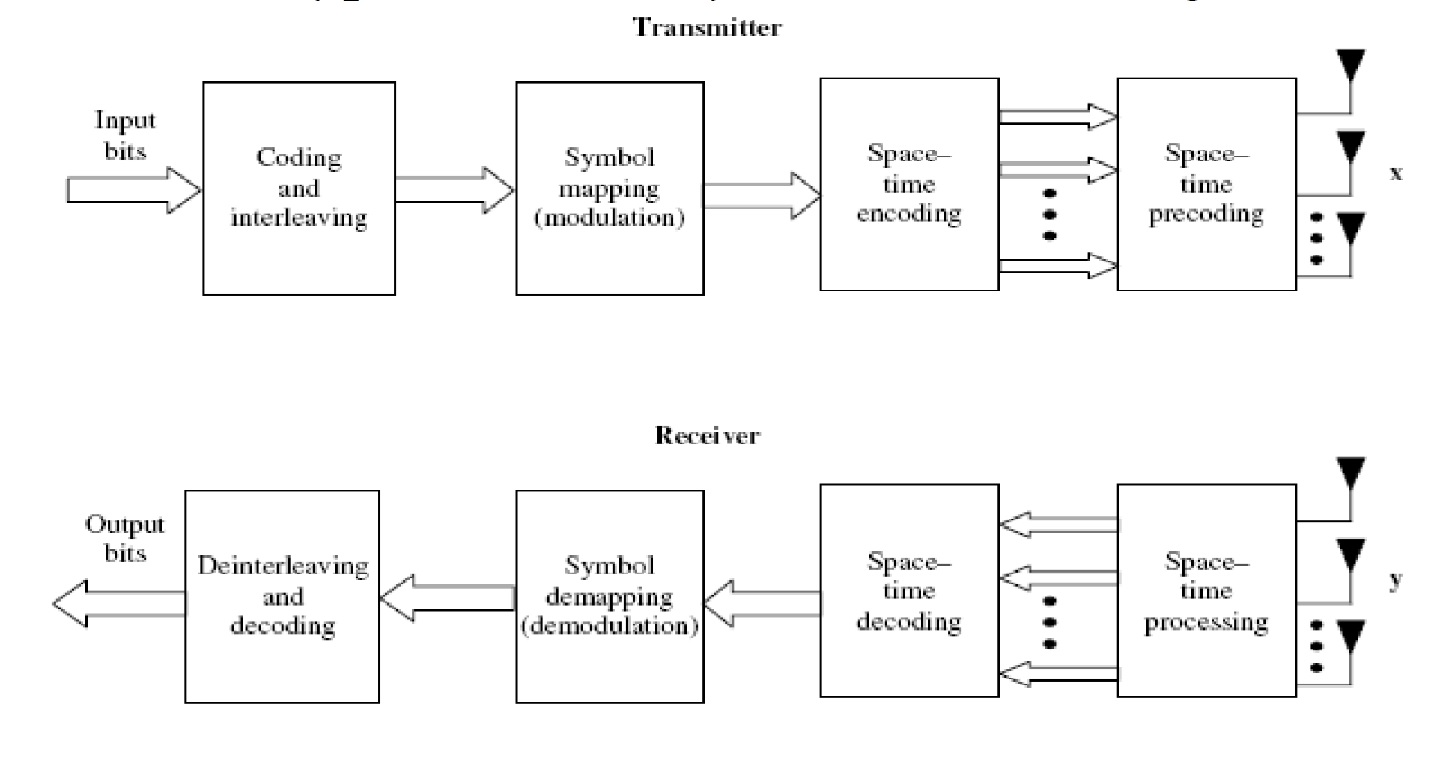
\includegraphics[width= 0.8\textwidth]{mimosystem.eps}
		\caption{MIMO System Model}
	\end{center}
\end{figure}


A typical \ac{MIMO} channel and system model equation is as represented as in equation 1. The wireless channel part can be seen in keenly with the received vector \me{y} can be represented in terms of the channel \me{H}. 

\begin{equation}
\mathbf{y} = H \mathbf{x} + n
\label{bgmimo1_eqn}
\end{equation}
where, transmitted signal vector \me{x = x_1,x_2, \dotsc,x_n}, recieved vector \me{y = y_1, y_2, \dotsc, y_n} and the channel matrix can be represented as, \me{H} =  \[ \left( \begin{array}{cccc} 
	h_{11} & h_{12} & \dotsc & h_{1M} \\
	h_{21} & h_{22} & \dotsc & h_{2M} \\
	\dotsc & \dotsc & \dotsc & \dotsc \\
	h_{N1} & h_{N2} & \dotsc & h_{NM} \end{array} \right)\].

The capacity for \ac{MIMO} network can be written as
\begin{equation}
C = \underset{f(x)}{\text{max}} I(X;Y) 
\label{bgmimo2_eqn}
\end{equation} 
where, \me{I(X;Y)} is the mutual information of the channel represented as,
\begin{equation}
I(X;Y) = \int \log (\dfrac{f(y|x)}{f(y)}) dF(x,y)
\label{bgmimo3_eqn}
\end{equation}
\begin{figure}[h]
	\begin{center}
		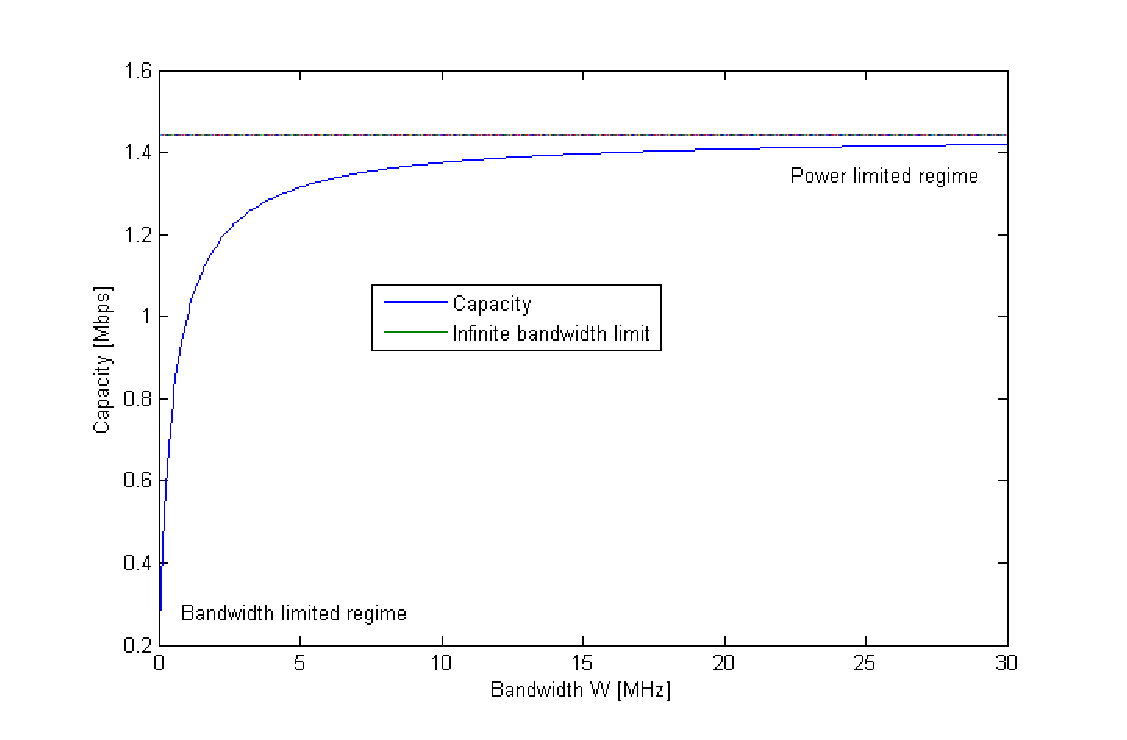
\includegraphics[width= 0.8\textwidth]{mimocapacity.eps}
		\caption{MIMO Capacity}
	\end{center}
\end{figure}
where the integral is taken over the random variables X and Y, \me{f(x)} and \me{f(y)} is denoted as the probability density function of X and Y, \me{F(x,y)} is the cumulative distribution function of X and Y respectively. The mutual Information can also be written in terms of differential output of channel entropy and the conditional entropy. 
\begin{equation}
I(X;Y) = h(Y) - h(Y|X)
\label{bgmimo4_eqn}
\end{equation}
For a time-invariant \ac{AWGN} channel with received \ac{SNR} \me{\gamma}, the maximizing input distribution is Gaussian, which results in the channel capacity	
\begin{equation}
C = \alpha \log (1 + \gamma)
\label{bgmimo5_eqn}
\end{equation}
 
At high \ac{SNR}, the capacity of the i.i.d. Rayleigh fast fading channel scales like \me{n_min \log} SNR bits/s/Hz, where \me{n_min} is the minimum of the number of transmit antennas \me{n_t} and receive antennas \me{n_r}. Thus, at high \ac{SNR} we obtain degree-of-freedom gain. At low \ac{SNR}, the capacity is approximately \me{n_r} SNR \me{\log_2}e bits/s/Hz. Thus at low \ac{SNR} what we obtain is the recieve beamforming power gain. At all \ac{SNR} the capacity increases linearly with \me{n_min} due to the linear combination of degree of freedom gain and beamforming power gain.

%The \ac{MIMO} information-theoretic performance bound of the system can be explained here while Capacity increases linearly at low \ac{SNR} but increases logarithmically at high \acs{SNR}. The linear region is the Bandwidth limited region and the logarithmic region is power limited region, since in low \ac{SNR} region the capacity which is defined as C = log (1 + SNR) where \ac{SNR} value is small so effectively we have log(1) like wise for high \ac{SNR} value the log(1 + SNR) term is effectively \ac{SNR} since for higher values log term increases slowly. 
%-----------------------------------------------------------------------------
%  MIMO ibc
%-----------------------------------------------------------------------------

\section{MIMO-IC}
\ac{MIMO} communication systems has been showing a great potential in increasing the average throughput in the wireless communication scenario. Due to the performance gain in channel capacity and spectral efficiency in point to point \ac{MIMO} systems has made the inclusion of singe user \ac{MIMO} in different communication stansards. SU-\ac{MIMO} has proved its efficiency to enhance the perormance in wireless networks. But, in cellular systems the available spectrum is very costly and is scarce so such systems has to deal with the inter-cell interference which doesnot exists in isolated point to point systems.

\begin{figure}[h]
	\begin{center}
		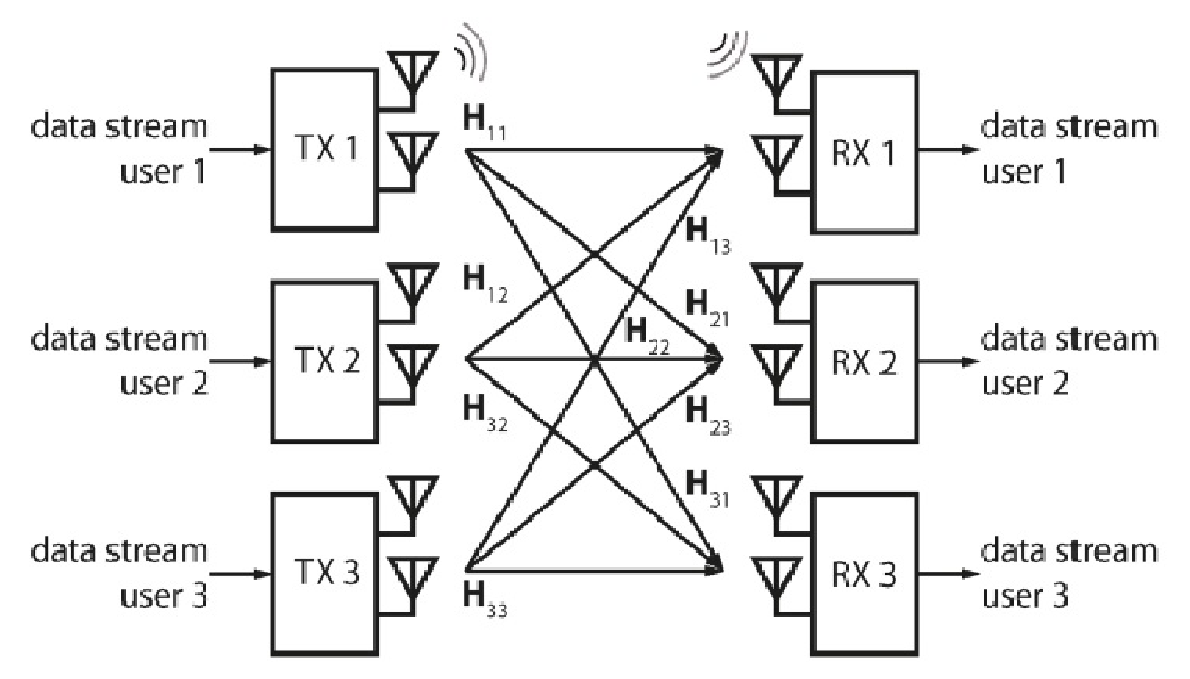
\includegraphics[width= 0.8\textwidth]{mimoibc.eps}
		\caption{MIMO-IC System Model}
	\end{center}
\end{figure}

Interference is a major set back and a limitting factor in the wireless communication networks. The problem of interference is in general  dealt  with  planning of the  (mostly  static) radio resource management. Now a days we have a popularity of wireless  devices  having  different  wireless  communication standards, the the ability to produce a desired or intended result of such interference avoidance solutions is limited. These days, standardization bodies are including  interference coordination strategies in  next generation  cellular  communication standards.  A  systematic study  of  the  performance of  cellular  communication systems where  each  cell  communicates  multiple  streams to  its  users while causing interference from and to the neighboring cells due  to  transmission  over  a  common  shared  resource  known as, \ac{MIMO}-\ac{IC}. A K-user \ac{MIMO}-\ac{IC} model consists of a network of K transmit-receive  pairs  where each transmitter  communicates  multiple data streams to its respective receiver. In doing so, it generates interference at all other receivers present in the system.




%-----------------------------------------------------------------------------
%  MIMO ibc
%-----------------------------------------------------------------------------


\section{MIMO-IBC}

The linear transceiver design problem is considered in a \ac{MIMO}-\ac{IBC}, in which a set of \ac{BS}s send data to their intended users. Both the \ac{BS}s and the users are equipped with multiple antennas, and they share the same time/frequency resource for transmission. The objective is to maximize the minimum rate among all the users in the network, in order to achieve fairness.

\begin{figure}[h]
	\begin{center}
		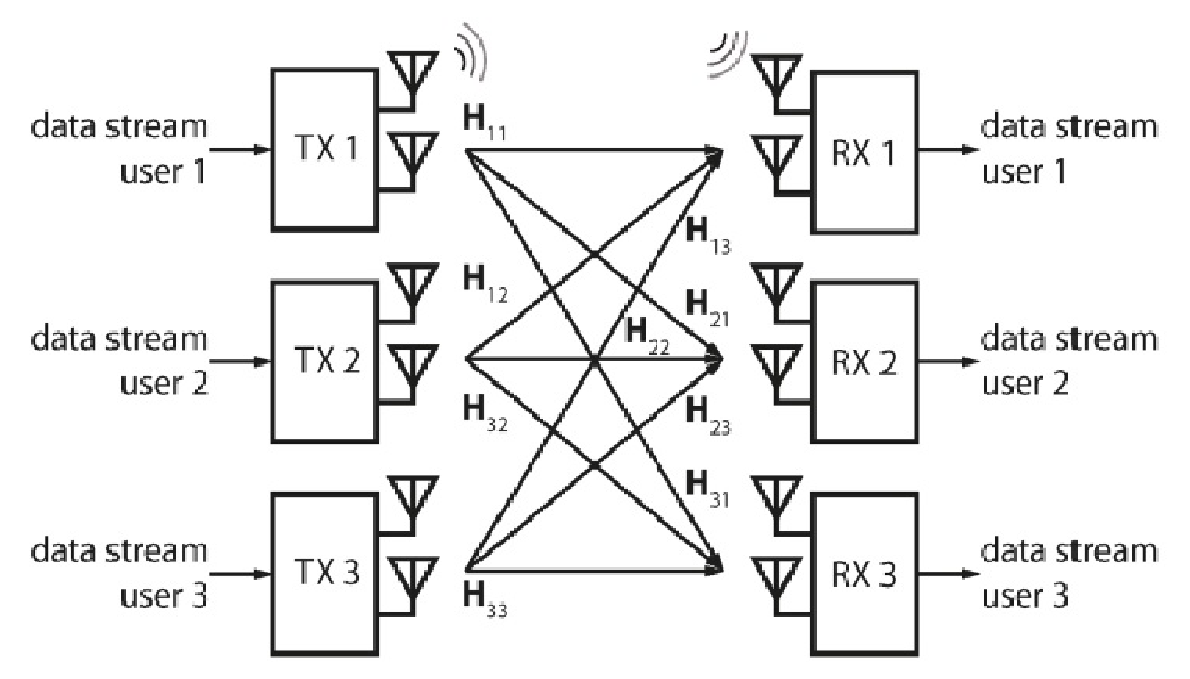
\includegraphics[width= 0.8\textwidth]{mimoibc.eps}
		\caption{MIMO-IBC System Model}
	\end{center}
\end{figure}

Interference is the main limiting factor in wireless transmission. \ac{BS} consisting of multiple antennas are able to serve multiple users simultaneously, which is the principle of \ac{SDMA} or \ac{MU-MIMO}. However, \ac{MU} systems have precise requirements for \ac{CSIT} which is more difficult to acquire than \ac{CSI} at the Rx \ac{CSIR}. Hence we focus here on the more challenging \ac{DL} (though the \ac{UL} is also non-trivial in the case of Mobile Terminals (MTs) with multiple antennas). In cellular systems, one can distinguish between the cell center where a single cell design is appropriate (due to high \ac{SIR} and the cell edge where a multi-cell approach is mandatory. The \ac{MU-MIMO} \ac{DL} problem for the cell center users is called the (MIMO) Broadcast Channel (BC). or the cell edge users,  the recent introduction of Interference Alignment (IA) has shown that approaching high system capacity through agressive frequency reuse should in principle be possible.  Whereas precise capacities for cellular systems remain unknown, IA allows to reach the optimal high \ac{SNR} rate prelog, called Degree of Freedom \ac{DoF} (or spatial multiplexing factor, or number of streams). That is, before accounting for \ac{CSI} acquisition.  

Optimal  precoder  design  for  \ac{WSRM} in \ac{MIMO} interference networks  is  studied.  For  this  well  known  non-convex  optimization problem, convex approximations based on interference alignment are developed, for multi-beam cases. Considering that each user treats interference from other users as noise. It is well known that, due to interference coupling, the problem is a non-convex optimization and is hard to solve. In the high \ac{SNR} regime, there has been recent progress on maximizing the sum degrees of freedom, exploiting the idea of interference alignment. It has been shown that maximizing the sum degrees of freedom is  still  an  NP  hard  problem. 


%-----------------------------------------------------------------------------
%  MATH
%-----------------------------------------------------------------------------


\section{Mathematical Preliminaries}
\subsection{Convex Optimization}
\subsubsection{Convexity}
Convexity is also called convex analysis, which is an area in mathematics where one studies about convex sets and convex functions. Convexity is also the mathematical core of optimization [1], where it plays an important role in statistics, differential equations and mathematical economics. Convexity can also be called as convex analysis. Some examples of convex sets are triangle, rectangle, polyhedron and quadratic equations.[1]. 
\begin{figure}[h]
	\begin{center}
		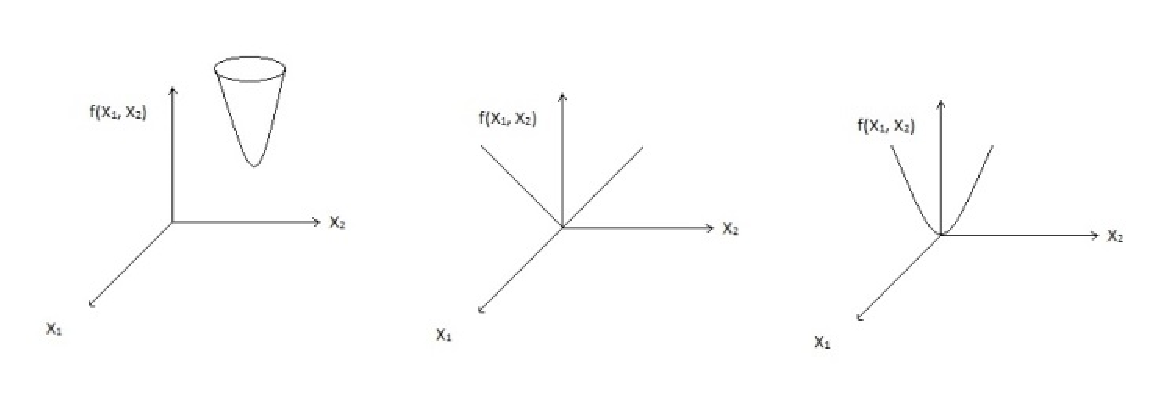
\includegraphics[width= 1.0\textwidth]{convexfunc.eps}
		\caption{Convex Functions}
	\end{center}
\end{figure}
\subsection{Convex Sets}
Consider \me{\mathcal{K}} is a set of \me{\mathcal{R}^n} is said to be convex when the line segment through the points \me{x, y} belongs to \me{\mathcal{K}}. In general, the points must lie inside the set and the set is connected such that without leaving the set we can pass through any two points. As mentioned above there are several examples for convex sets like ellipsoid, hypercubes etc. We can also define that the intersection of any convex sets is a convex set.[2]. 
A set that is not convex is called non convex set or also called as concave set. We can define a non convex set by considering a line segment joining the points \me{x, y} lies outside the set \me{\mathcal{K}}.
\begin{figure}[h]
	\begin{center}
		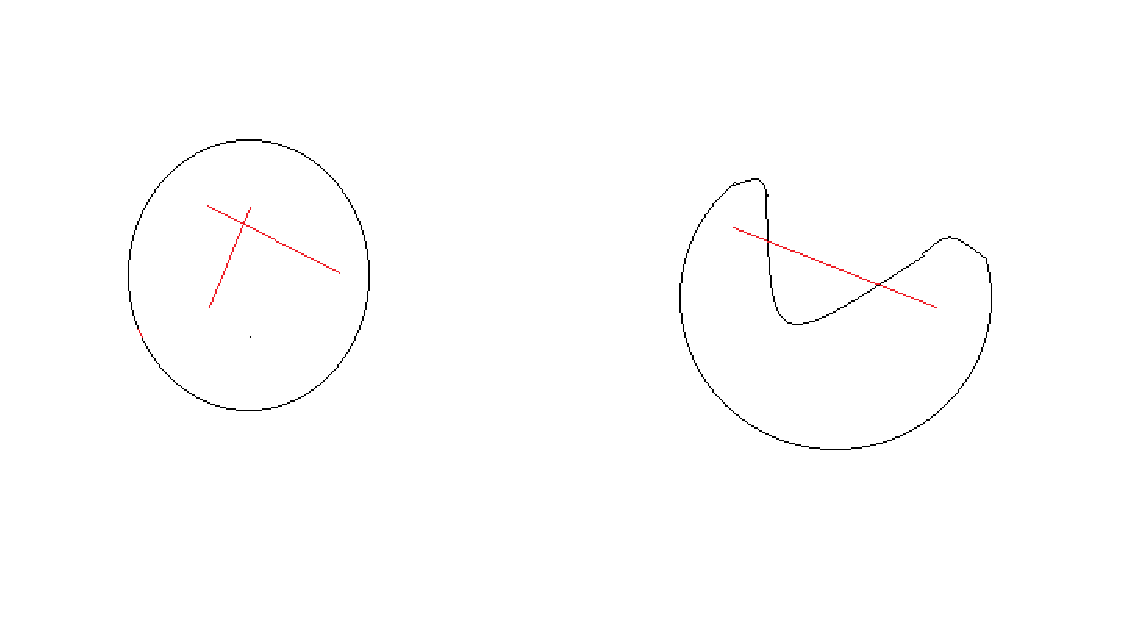
\includegraphics[width= 0.8\textwidth]{convexset.eps}
		\caption{Convex Sets}
	\end{center}
\end{figure}

\subsubsection{Convex Functions}

Convex functions are continuous function and is convex if and only if the region above the graph as shown in figure is convex set. A function \me{f} is convex if, \me{\forall} \me{x, y} \me{\in} \me{\mathcal{K}}, \me{ \forall} \me{ \theta \in} [0, 1]: 
\begin{equation}
f(\theta x + (1 - \theta) y) \leq \theta f(x) + (1 - \theta) f(y)
\end{equation}
The function \me{f} is said to be strictly convex if, \me{ \forall} \me{x \neq y} \me{\in} \me{\mathcal{K}}, \me{ \forall} \me{ \theta \in} (0, 1):
\begin{equation}
f(\theta x + (1 - \theta) y) < \theta f(x) + (1 - \theta) f(y)
\end{equation}
A function \me{f} is said to be concave if the function -\me{f} is strictly convex. Strict convexity means that the graph of \me{f} lies below the segment \me{\mathcal{S}}. Certain examples of strict convex functions are exponential and quadratic function. Several operations on these function preserves the convexity like summation, multiplication of convex functions. 

\subsubsection{Optimization Problem}

A generic optimization problem is similar to linear programming problem, that can be solved quickly depending on the variables and the constraints. The objective and the constraints must be linear for the problem to be convex. In general, a convex optimization problem has all of the constraints as convex functions, and the objective is a convex function of minimizing, or a concave function of maximizing. 

The standard form of optimization problem can be written as,
\begin{eqnarray}
\underset{x}{\text{minimize}} \quad && f(x) \\
\text{subject to} \quad && x \in \mathcal{X}. 
\end{eqnarray}
where, \me{f(x): {\mathbb{R}^n} \rightarrow {\mathbb{R}}} is the objective function that has to be minimized with respect to \me{x} and \me{\mathcal{X}} \me{\subset} \me{{\mathbb{R}^n}} is the feasible set. A maximization problem can be written by negating the objective function.

\subsubsection{Convex Problem}

A convex optimization problem is one which has both the objective and the given set of constraint as convex. In general linear functions are convex so the linear programming problem is convex problem. A general convex optimization problem can be written as
\begin{eqnarray}
\underset{x}{\text{minimize}} \quad && f(x) \\
\text{subject to} \quad && g_i(x) \leq 0, i = 1,...m\\
&& h_j(x) = 0, j = 1,...p.
\end{eqnarray}
where, \me{f(x): {\mathbb{R}^n} \rightarrow {\mathbb{R}}} is the objective function and \me{\mathcal{X}} \me{\subset} \me{{\mathbb{R}^n}} is the feasible set and is called convex when \me{\mathcal{X}} is closed convex set and \me{f(x)} is convex on \me{{\mathbb{R}^n}}. The second equation is the inequality constraint and the third is the equality constraint in the above optimization problem.
\par
The optimality condition for a convex problem; assume a feasible point \me{\mathbf{x}^*} but it is necessary to know if this point is the optimal solution. We can consider the gradient of a function \me{f} that shows the ascent direction of the function. Gradient of \me{f} at a point \me{x} divides the space into three regions one where the function increases, one where the function decreases and the one where we cannot figure out using the gradient alone. For \me{\mathbf{x}^*} to be optimal and the feasible region doesn't lie in the half space where the function decreases, if not then the point \me{\mathbf{x}^*} is not the optimal point. Convexity makes this condition sufficient for optimality. 
\par
To find solution for an unconstrained objective, we differentiate the objective function with respect to the optimization variable \me{x} and equate to zero as \me{\nabla f(x) = 0}. However for an constrained problem, we solve the Lagrangian as
\begin{equation}
\underset{\lambda}{\text{maximize}} \quad \underset{x}{\text{minimize}} \quad  L(x,\lambda_1, \dotsc,\lambda_m) =  f(x) + \lambda_1 g_1(x) + \dotsc + \lambda_m g_m(x) + \mu_1 h_1 (x) + \dotsc + \mu_p h_p(x),
\end{equation}
where \me{\lambda_i \geq 0} and \me{\mu_j} are Lagrange multipliers. In order to solve the constrained problem, similar to the unconstrained problem we take the partial derivative of the Lagrangian with respect to the optimization variable.
\par
When the objective is convex, and the equality conditions are affine and the inequality conditions are convex then one of the possible solutions, in some minimum principle is equivalent to \ac{KKT} optimality conditions. To solve a convex optimization problem as above with the \ac{KKT} approach we need the lagrange multiplier. There exists \me{\lambda_1, \lambda_2, \dotsc, \lambda_m, \mu_1, \dotsc, \mu_p}, called the Lagrange multipliers, for each point \me{x \in X} that minimizes f over \me{\mathcal{X}}. The Lagrange multipliers must satisfy certain conditions:\\
 1. \me{{x} \quad minimizes \quad L(z, \lambda_1, \lambda_2, \dotsc, \lambda_m),   \forall z \in X},\\
 2. \me{\lambda_1 \geq 0, \lambda_2 \geq 0, \dotsc, \lambda_m \geq 0},\\
 3. Complementary Slackness: \me{\lambda_1 g_1 = 0, \lambda_2 g_2 = 0, \dotsc, \lambda_m g_m = 0}.\\
\par 
When the problem is has a convex objective and non convex constraint set then \ac{KKT} method is not a feasible approach. 


\subsubsection{Non Convex Problem}
 
A non convex problem is the one that has objective or any one of its constraint as non convex. Such problems have multiple feasible regions and multiple local minima in a region. An example for a non convex function would be a sine wave. Let us consider a non convex problem,
\begin{eqnarray}
\underset{x}{\text{minimize}} \quad && f(x) \\
\text{subject to} \quad && g_i(x) \leq 0, i = 1,\dotsc,m\\
&& h_j(x) = 0, j = 1,\dotsc,p.
\end{eqnarray} 
with variable \me{x \in \mathbb{R}^n}
\par
Let us consider a non convex problem when the objective function \me{f(x)} is convex and the inequality constraint \me{g_i(x)}, \me{i=1,\dotsc,n}  is differentiable convex function and \me{g_i(x)}  \me{i= (n+1),\dotsc,m} are differentiable function and the linearity constraint is affine. These non convex problems are common in wireless communication and this is our interest. In order to solve this problem the non convex part of the objective is approximated around a convex function to solve in an iterative manner. 
\par
As mentioned in the paper gordon.p. wright the inner approximation algorithm for the minimization problem can be done in the following steps,\\
\par
step 0. Set a starting point for the variable and constraint \me{x^0 \in F} and set \me{h^0 = g_0(x^0)}. Let \me{A^0 = \lbrace x|h^0 = g_0(x)} and \me{x \in F \rbrace}, where \me{F} can be defined as the feasible region.\\
\par
step 1. In the \me{k^{th}} iteration replace the constraint \me{g_i(x) \leq 0}, \me{i = (n+1), \dotsc, m}, by \me{\bar{g_i}(x,x^k) \leq 0}, where \me{\bar{g_i}(x,x^k)} is a differentiable convex function and \me{x^k \in \mathcal{A}^{k - 1}}. Each function \me{\bar{g_i}(x,x^k)} must  have the following properties,\\
1. \me{g_i(x) \leq \bar{g}_i(x,x^k) \quad \forall x \in {F}^k}\\
2. \me{g_i(x) = \bar{g_i(x^k,x^k)}}\\
3. \me{\delta g_i(x^k)/ \delta x_j =\delta \bar{g}_i(x^k,x^k)/\delta x_j \quad j=1,\dotsc,n}\\
The feasible region \me{F^k = \lbrace x|g_i(x) \leq 0 \forall i= 1,\dotsc , n} and \me{\bar{g}_i(x,x^k) \leq 0 \forall i= n+1, \dotsc, m \rbrace} should satisfy slaters constraint qualification condition for convex programs.\\
\par
step 2. Solve the approximation convex program\\

\begin{eqnarray}
\underset{x}{\text{minimize}} \quad && g_0(x) \\
\text{subject to} \quad && g_i(x) \leq 0, i = 1,\dotsc,n\\
&& \bar{g}_i(x,x^k) \leq 0, i = n + 1,\dotsc,m.
\end{eqnarray} 
Let \me{h^k = min \lbrace g_0(x)|x \in F^k \rbrace}.\\
\par
step 3. If \me{h^k = h^(k-1)}, then \me{x^k} is a \ac{KKT} solution for the minimization problem. Otherwise, let \me{a^k = \lbrace x|h^k = g_0(x)} and \me{x \in F^k \rbrace} and return to step 1.\\
\par
The above algorithm proposed by WRIGHT can be used to optimize non linear programs even when the constraint is a non convex function. The objective is replaced with a new variable and is added into the constraint set. As mentioned in the paper, the solution for the algorithm is not only the \ac{KKT} point but also the global minimum for approximating convex problem that is interior to the feasible region.



%-----------------------------------------------------------------------------
% Precoder
%-----------------------------------------------------------------------------



\chapter{Precoder Design} 

\section{Introduction to Precoder design}

Precoding can be explained as the beamforming method used for multi-stream transmission in \ac{MIMO} communication. Multiple data streams are emitted from the transmit antenna having weights to maximize the throughput of receiver output. In this technique, transmitter sends coded information to the receiver for analyzing the channel, where the receiver is a simple detector, example a matched filter, and does not need the channel side information. Thus reducing the effects of channel used for the communication. Precoding can be explained for both point to point systems and multi-user \ac{MIMO} system.

In point-to-point \ac{MIMO} system, transmitter is equipped with multiple antennas that communicates with a receiver that has multiple antennas. The precoding in point to point case assumes a narrowband slowly fading channel, that is achieved through \ac{OFDM}, and the channel capacity and throughput can be maximized depending on the \ac{CSI} available in the system. If the transmitter has statistical information and the receiver knows the channel matrix then eigen beamforming achieves the \ac{MIMO} channel capacity, where, the transmitter emits multiple streams in eigen directions of the channel covariance matrix. If the channel matrix is completely known, singular-value-decomposition \ac{SVD} precoding is known to achieve the \ac{MIMO} channel capacity, where, the channel matrix is diagonalized by taking an \ac{SVD} and removing the two unitary matrices through pre- and post-multiplication at the transmitter and receiver, respectively, thus, one data stream per singular value can be transmitted without having any interference.

In \ac{MU-MIMO}, a multi-antenna transmitter communicates simultaneously with multiple receivers with one or more antennas known as \ac{SDMA}. Precoding algorithms for \ac{SDMA} systems can be sub-divided into linear and nonlinear precoding types. The capacity achieving algorithms are nonlinear approach but linear precoding approaches usually achieve reasonable performance with much lower complexity. Linear precoding strategies include \ac{MRT},  \ac{ZF} precoding, and transmit Wiener precoding, there are also precoding strategies for low-rate feedback of channel state information. Nonlinear precoding is designed based on the concept of \ac{DPC}, which shows that any known interference at the transmitter can be subtracted without the penalty of radio resources if the optimal precoding scheme can be applied on the transmit signal.

\ac{DPC} is a coding technique that pre-cancels known interference without power penalty. Only the transmitter needs to know this  interference, but full \ac{CSI} is required everywhere to achieve the weighted sum capacity. \ac{DPC} is known as the capacity achieving scheme in the \ac{MIMO} channel. But \ac{DPC} is a Non-linear technique for interference cancellation having higher degree of complexity. Thus, to overcome this we can go for a linear technique considering the problem of  \ac{WSRM} with linear transmit precoding for multicell  \ac{MIMO} downlink. But, the \ac{WSRM} problem, for single-antenna receivers are considered to be NP-hard. Although 
optimal beamformers can be obtained and they may not be practically useful since the complexity of finding optimal designs grows exponentially with the problem size. Hence, the need of computationally conducive suboptimal solutions to the WSRM problem 
still remains. Since the \ac{WSRM} problem is nonconvex and NP-hard, there exists a class of beamformer designs which 
are based on achieving the necessary optimal conditions of the \ac{WSRM} problem.


%--------------------------------------------------------------------
%sys model precoder design-------------------------------------------
%--------------------------------------------------------------------

\subsection{System Model}

Consider a downlink \ac{MIMO} \ac{IBC} system with \me{\mathcal {B}} coordinated \ac{BS} of N transmit antennas each and \me{K} single antenna receivers. The set of all \me{K} users is denoted by \me{\mathcal{U} = \{1,2,\dotsc, K\}}. We assume that data for the \me{k^{th}} user is transmitted only from one BS, which is denoted by \me{b_k \in \mathcal{B}}, where \me{\mathcal{B} \triangleq \{1,2,\dotsc, \mathcal{B}\}} is the set of all \ac{BS}. The set of all users served by BS \me{b} is denoted by \me{\mathcal{U}_b}. Under flat fading channel conditions, the input-output relation for \me{k^{th}} user is given as
\begin{equation}
y_k = \mathbf{h}_{b_k,k}^H \mathbf{x}_k  + {n}_k
\label{precoder1_eqn}
\end{equation}
where \me{h_k} is the channel coefficient showing the channel response between transmit and recieve antenna, ie., from \ac{BS} \me{b} to user \me{k} and \me{{n} \thicksim \mathcal{CN}(0,\sigma^{2})} is complex circularly symmetric zero mean gaussian noise with variance  \me{\sigma^2}. The receiver requires information about the channel \me{h_k} to suppress the effect of noise \me{n}. By doing this, complexity is increased, but the receiver has to be simple that, the \ac{BS} can predict the channel.

Under linear precoding the transmitted vector \me{x} can be written as
\begin{equation}
\mathbf{x}_k = \sum^K_{i=1} \mathbf{w}_i d_i
\label{precoder2_eqn}
\end{equation}
where, \me{d_i} is normalized data symbol and \me{w_i} is the linear precoding vector. The \ac{SINR} (\me{\gamma_k}) can be written as
\begin{equation}
\gamma_k = \frac{ \|\mathbf{h}_{b_k,k} \mathbf{w}_k\|^{2}}{\sigma^{2}+\sum_{i = 1, i \neq k}^{K} \|\mathbf{h}_{b_i,k} \mathbf{w}_{i}\|^{2}}
\label{precoder3_eqn}
\end{equation}

For reliable communication achievable commuinication rate can be written as
\begin{equation}
C = \mathbf{log}_2(1 + \gamma_k) 
\label{precoder4_eqn}
\end{equation}
where, C is the achievable capacity. The transmission is power limited with a total power constraint as
\begin{equation}
\sum_{i = 1}^{K} \|\mathbf{w}_i\|^2 \leq \mathbf{P}.
\label{precoder5_eqn}
\end{equation} 

The precoder design can be classified into Centralized and Distributed approach. In the centralized approach all the \ac{BS} share the \ac{CSI}. The centralized controller is equipped to know and calculate the expected sum rate. In distributed approach, practical difficulties of distributing \ac{CSI} over the backhaul network and high complexity of joint precoding design motivates the analysis. The beamforming and power allocation strategies can be computed locally using only local \ac{CSI} in a distributed design. In general, the goal of precoding is to maximize the signal power at the intended terminal while minimizing the interference caused at others. 




\newpage
%-----------------------------------------------------------------------------
%  centrl PRECODER DESIGN
%-----------------------------------------------------------------------------


\chapter{Centralized Precoder Design}

A centralized coordinated \ac{DL} transmission requires \ac{CSI} to be feedback from the users to their serving \ac{BS}, and aggregated at the central coordination node to form the channel matrix for precoding, so that interference can be mitigated.

%--------------------------------------------------------------------
%sys model precoder design-------------------------------------------
%--------------------------------------------------------------------

\section*{System Model for \ac{WSRM} }

Consider a downlink \ac{MIMO} \ac{IBC} system with \me{\mathcal {B}} coordinated \ac{BS} of N transmit antennas each and \me{K} single antenna receivers. The set of all \me{K} users is denoted by \me{\mathcal{U} = \{1,2,\dotsc, K\}}. We assume that data for the \me{k^{th}} user is transmitted only from one BS, which is denoted by \me{b_k \in \mathcal{B}}, where \me{\mathcal{B} \triangleq \{1,2,\dotsc, \mathcal{B}\}} is the set of all \acsp{BS}. The set of all users served by BS \me{b} is denoted by \me{\mathcal{U}_b}. Under flat fading channel conditions, the signal received by the \me{k^{th}} user is
\begin{equation}
h_k{x}_k = \mvecH{w}{k} \mathbf{h}_{{b_k},k} \mathbf{x}_k  + \mathbf{w}^H_k \sum_{i = 1, i \neq k}^{K} \mathbf{h}_{{b_i},k} \mathbf{x}_i + \mathbf{w}^H_k \mathbf{n}_k
\label{cent1_eqn}
\end{equation}

where \me{\mvec{h}{b_i,k} \in \mathbb{C}^{1 \times N}} is the channel (row) vector from BS \me{{b_i}} to user \me{{k}, \mathbf {w}_k \in \mathbb{C}^{N \times 1}} is the beamforming vector (beamformers) from BS \me{{b}_k} to user \me{{k}}, \me{{d}_k} is the normalized complex data symbol, and \me{{n}_k \thicksim \mathcal{CN}(0,\sigma^{2})} is complex circularly symmetric zero mean gaussian noise with variance \me{\sigma^2}. The term \me{\textstyle \sum_{i = 1, i \neq k}^{K} \mathbf{h}_{{b_i},k} \mathbf{w}_i d_i} in \eqref{rx_eqn} includes both intra- and inter-cell interference. The total power transmitted by \acs{BS} \me{b} is \me{\textstyle \sum_{k \in \mathcal{U}_b} \|\mathbf{w}_k\|^{2}}. The \acs{SINR} \me{\gamma_k} of user \me{k} is
\begin{equation}
\gamma_k = \frac{ \|\mvec{h}{b_k,k} \mathbf{w}_k\|^{2}}{\sigma^{2}+\sum_{i = 1, i \neq k}^{K} \|\mathbf{h}_{{b_i},k}\|}
\label{cent2_eqn}
\end{equation}

Here, we are interested in the problem of \acs{WSRM} under per-\ac{BS} power constraints, which is formulated as
\begin{equation}
\max_{\sum_{k \in \mathcal{U}_b} \| \mathbf{w}_k \|^2 \leq {P_b}, \forall \, b \in \mathcal{B} }  \quad \sum_{k = 1}^{K} \alpha_k \log(1 + \gamma_k)
\label{cent3_eqn}
\end{equation}
where \me{\alpha_k}'s are positive weighting factors which are typically introduced to maintain a certain degree of fairness among users.

%--------------------------------------------------------------------
%prb frmlatn precoder design-----------------------------------------
%--------------------------------------------------------------------

\section*{Problem Formulation}

To achieve a tractable solution for the Low-Complexity beamfomer design, we can write the problem as shown in the following equation,

\begin{equation}
\max_{\sum_{k \in \mathcal{U}_b} \| \mathbf{w}_k \|^2 \leq {P_b}, \forall {b \in \mathcal{B}} }  \quad          \prod_{k} (1 + \gamma_k)^{\alpha_k}
\label{cent4_eqn}
\end{equation}

The equations can be re-written as
\begin{subeqnarray}
	\displaystyle \max_{w_k, t_k} \quad && \prod_{k} t_k \slabel{cent5c_eqn}\\
	\text{subject to} \quad && \gamma_k \geq {t_k}^{1/\alpha_k} - 1 , \forall k \in \mathcal{U}, \slabel{cent5a_eqn} \\
	&& \sum_{k \in \mathcal{U}_b} \| \mathbf{w}_k \|_2^2 \leq {P_b}, \forall {b \in \mathcal{B}}. \slabel{cent5b_eqn}
	\label{cent5_eqn}
\end{subeqnarray}

In equation \eqref{cent5a_eqn} and \eqref{cent5b_eqn} it can be seen that all constraints are active at the optimum, otherwise, we can obtain a larger objective by increasing \me{t_k} without violating the constraints. We can reformulate \eqref{cent5a_eqn} by reintroducing additional slack variable \me{\beta_k},

\begin{subeqnarray}
	\underset{w_k, t_k, \beta_k}{\text{maximize}} \quad && \prod_{k} t_k \\
	\text{subject to} \quad && \Re {\mathbf{h}_{{b_k},k} \mathbf{w}_k} \geq \sqrt{{t_k}^{1/\alpha_k} - 1 } \beta_k , \forall k \in \mathcal{U} \slabel{cent6a_eqn}\\
	&& \Im (\mathbf{h}_{{b_k},k} \mathbf{w}_k) = 0, \forall k \in \mathcal{U}, \slabel{cent6b_eqn} \\
	&& ({{\sigma^{2}+\sum_{i = 1, i \neq k}^{K} \|\mathbf{h}_{{b_i},k}\mathbf{w}_k}\|^{2}})^{1/2} \leq \beta_k, \forall k \in \mathcal{U}, \slabel{cent6c_eqn} \\
	&& \sum_{k \in \mathcal{U}_b} \| \mathbf{w}_k \|_2^2 \leq {P_b}, \forall {b \in \mathcal{B}}. \slabel{cent6d_eqn}
	\label{cent6_eqn}
\end{subeqnarray}

The relation between \eqref{cent5a_eqn} and \eqref{cent6b_eqn} can be seen as, first, by forcing the imaginary part of \me{\mathbf{h}_{{b_k},k} \mathbf{w}_k} to zero in \eqref{cent6b_eqn} does not affect the optimality of \eqref{cent5b_eqn} since phase rotation on \me{\mathbf{w}_k} will result in the same objective while satisfying all constraints. Second we can show that all the constraints in \eqref{cent6_eqn} hold with equality at the optimum.


\newpage

 

\newpage





%-----------------------------------------------------------------------------
% ADMM
%-----------------------------------------------------------------------------

\chapter{Distributed Precoder Design} 

In the distributed precoder design, the precoders are designed independently at each \ac{BS}. The convex formulation in the above equation requires a centralized controller to perform the precoder design for all users belonging to the coordinating \ac{BS}s. To design the precoders independently at each \ac{BS} with lesser information exchange via backhaul, iterative decentralized methods are used. In general, the decentralized approaches are mainly based on primal or the alternating method of multipliers \ac{ADMM} schemes. 

\section*{Problem Formulation}

We consider the convex sub problem with fixed receive beamformers \me{w_k} based on Taylors series approximation for the non convex constraint. The objective function of equation \eqref{cent5c_eqn} can be decoupled across each \ac{BS} as 
\begin{subeqnarray}
\sum_k \log(1 + \gamma_k) \geq \log(1 + \gamma_k)\\
\prod_k (1 + \gamma_k) \geq (1 + \gamma_k)
\end{subeqnarray}
thus the centralized problem can be represented in equivalent form as
\begin{subeqnarray}
\underset{w_k, \beta_k}{\text{maximize}} \quad && \sum_{k=1}^{K} \log(1 + \gamma_k)  \\
\text{subject to} \quad && \eqref{cent6a_eqn} - \eqref{cent6d_eqn}
\end{subeqnarray}
where, \me{\log(1+\gamma_k)} represents the vector of weighted sum of users \me{k \in \mathcal{U}_b}. Let us consider \me{\mathcal{U}_b} as, the users from my \ac{BS} and \me{\mathcal{U}_{\bar{b}}} as the users from the interfering \ac{BS}. The set of all \me{K} users is denoted by \me{\mathcal{U} = \{1,2,\dotsc, K\}}. We assume that data for the \me{k^{th}} user is transmitted only from one BS, which is denoted by \me{b_k \in \mathcal{B}}, where \me{\mathcal{B} \triangleq \{1,2,\dotsc, \mathcal{B}\}} is the set of all \ac{BS}. The set of all users served by BS \me{b} is denoted by \me{\mathcal{U}_b}. 

The problem can be decentralized or distributed with the \ac{BS} specific interference vector term, which can be fixed or can be used as a variable depending on the choice of our decomposition method. The given convex problem can be decomposed to parallel iterative subproblems cordinated by primal or dual decomposition update. The coupling variables are updated in each iteration by interchanging the given information within the subproblem. 

\section{Primal and Alternating Direction Method of Multipliers (\acs{ADMM}) Schemes}

In the Primal decomposition method, the convex problem can be solved for optimal transmit precoders in an iterative manner for fixed \ac{BS}. Using a master-slave model the problem can be solved, where the slave problem is solved in the corresponding \ac{BS} for optimal tranmit precoders. Upon finding the 
optimal transmit precoder in the subproblem, the master problem is used to update the \ac{BS} specific interference term for the next iteration by using the dual variables corresponding to the interference constraint. Thus these steps are continued further until a global optimal solution is obtained. The primal problem is similar to the minimum power precoder design as shown in paper "g. scutari". Hence, the master problem treats the interference term as variable where as, in the slave the interference term is considered as a constant for every iteration. 


The \ac{ADMM} method is used to decouple the precoder design across multiple \ac{BS}s inorder to solve the convex problem. In contrary with the primal decomposition method,  dual composition method reduces the constraint by considering the objective functions in the sub problem. The \ac{ADMM} approach is prefered over dual decomposition method due to its robustness and improved convergence. In this method we hold a local and a global copy of the signal interference. At optimality the copies remain equal.
\acs{ADMM} method can be formulated as following,

\begin{subeqnarray}
\underset{\substack{w_k, t_k, \beta_k, \\ \delta^{b_k}_{b,k}, \delta^{b_k}_{b_k,i}}}{\text{maximize}} \quad && \sum_{k} \log {t_k} +\sum_{k \in \mathcal{U}_{b_k}}\sum_{b \in {\bar{\mathcal{B}}}_{b_k}} \lambda^{b_k}_{b,k}{( {\delta ^{b_k}_{b,k} - \delta^G_{b,k} })}+ \sum_{i \in {\bar{\mathcal{U}}_{b_k}}} \lambda^{b_k}_{b_k,i}{( {\delta ^{b_k}_{b_k,i} - \delta^G_{b_k,i}})} - \nonumber \\
&&{\frac \rho {2}} \sum_{k \in \mathcal{U}_{b_k}}\sum_{b \in {\bar{\mathcal{B}}}_{b_k}}\|\delta ^{b_k}_{b,k} - \delta^G_{b,k} \|^{2}_{2}-{\frac \rho {2}}\sum_{i \in {\bar{\mathcal{U}}_{b_k}}} \|\delta ^{b_k}_{b_k,i} - \delta^G_{b_k,i} \|^{2}_{2} \\
\text{subject to} \quad && \mathbf{h}_{{b_k},k} \mathbf{w}_k \geq \beta_k  \sqrt{({t_k}^{1/\alpha_k} - 1) } , \forall k \in \mathcal{U}_{b_k} \slabel{8b_eqn}\\
        && \mathrm{Im}(\mathbf{h}_{{b_k},k} \mathbf{w}_k) = 0, \forall k \in \mathcal{U}_{b_k}, \slabel{8c_eqn} \\
        && {{\sigma^{2}+\sum_{\substack{i \in \mathcal{U}_{b_k} \\i \neq k}} \|\mathbf{h}_{{b_k},k}\mathbf{w}_i}\|^{2}}+\sum_{b \in {\bar{\mathcal{B}}}_{b_k}} \delta ^{(b_k)}_{b,k}  \leq \beta_k, \forall k \in \mathcal{U}_{b_k}, \slabel{8d_eqn} \\
        &&\delta ^{(b_k)}_{b,j} \geq \sum_{i \in {\mathcal{U}}_{b}} \|\mathbf{h}_{{b_k},k}\mathbf{w}_i\|^{2}, \slabel{8e_eqn} \forall j \in {\bar{\mathcal{U}}}_{b_k} \\
        && \sum_{k \in \mathcal{U}_b} \| \mathbf{w}_k \|_2^2 \leq {P_b}, \forall {k \in \mathcal{U}_{b_k}}. \slabel{8f_eqn}
\label{8_eqn}
\end{subeqnarray}

In the equation above the objective function of the precoder design is to maximize the sum rate (WSRM)problem. The ADMM method uses the sub gradient update method, where we assume the interference term from the adjascent BS. The \me{\delta ^{(b_k)}} is the local interference term taken into account from the adjascent BS, similarly the \me{\delta ^{(G)}} is the global interference term taken into account from the adjascent BS.At optimality the local and the global interference terms becomes same. The equation \eqref{8b_eqn} and the equation \eqref{8c_eqn} remains the same as the previous formulation. In the equation \eqref{8d_eqn} we observe that there is the local interference term coming from the adjascent BS adding into the noise plus the interference from the same BS. Similarly equation \eqref{8e_eqn} shows the sum of all interefrence terms from the adjascent BS.

\begin{algorithm}[h]
	\caption[Distributed Precoder Design]{ADMM Method}
	\label{algo-1}
	\begin{algorithmic}
		\label{algo--1}
		\STATE \textbf{Input:} \me{\alpha_k, \mathbf{h}_{b_k,k}, \forall b \in \mathcal{B}, \forall k \in \mathcal{U}_b}.
		\STATE \textbf{Output:} \me{\mathbf{w}_k, \forall k \in \lbrace{1,2,\dotsc,K \rbrace}}
		\STATE \textbf{Initialization:} \me{i = 0} and \me{\mathbf{w}_k} satisfying (5.5f)\\
		precoders randomly satisfies the power constant \me{\sum_{k \in \mathcal{U}_b} \| \mathbf{w}_k \|_2^2 \leq {P_b}, \forall {k \in \mathcal{U}_{b}}}
		\STATE initialize global interference vector \me{\delta^{(0)} = 0^T}
		\STATE initialize interference threshold \me{\lambda \forall b \in \mathcal{B}}\\
		\STATE \textbf{for each} \ac{BS} \me{b \in \mathcal{B}} perform the following procedure
		\REPEAT 
		\STATE initialize \me{j = 0} 
		\REPEAT	
		\STATE solve the precoders \me{\mathbf{w}_k} and local interference \me{\delta^{{b_i},k}} using the equation.
		\STATE exchange \me{\delta^{b}} across the co-ordinating \ac{BS} \me{\mathcal{B}}
		\STATE update dual variable \me{\lambda} using equation
		\STATE update the global interference
		\UNTIL {convergence \me{j \geq J_{max}}}\\
		\STATE update the beamformer \me{\mathbf{w}_k} with the recent precoder.\\ 
		\STATE exchange the receive precoder \me{\mathbf{w}_k \forall k \in \mathcal{U}_b} among the \ac{BS}.\\
		Update \me{\beta_k} with the precoder \me{\mathbf{w}_k}
		i=i+1
		\UNTIL {convergence \me{i \geq I_{max}}}
	\end{algorithmic} 
\end{algorithm}

Let us consider a two base station scenario such that the global interference term can be updated as follows,

\begin{equation}
\delta ^ {G}_{b,k} ={ \frac 1 {2}}{(\delta^{(b)}_{b,k}+\delta^{(b_k)}_{b,k})}
\label{deltaupdate_eqn}
\end{equation}

where \me{\delta^{(b)}_{b,k}} refers to the actual interference caused by BS \me{b} and \me{\delta^{(b_k)}_{b,k}} refers to the local interference caused by the BS \me{b_k}.

The update for the local interference term is made through iteration of the objective function in each BS. Once the local interference iterations are done then the global interference and the dual variable update are made in the main problem. The dual variable corresponds to the interference terms in the BS \me{b_k} and is updated with the sub gradient method. \me{\rho} gives the dual update step length depending upon the system performance and convergence behaviour. The convergence nature  of the distributed algorithm depends upon the choice made on step size. The distributed precoder design based on \ac{ADMM} is shown in Algorithm 1. The convergence for distributed algorithm is discussed in the Appendix

\begin{equation}
\lambda ^ {(n+1)}_{b,k} = \lambda ^ {(n)}_{b,k} - \rho{(\delta^{(b_k)^*}_{b,k}-\delta^{(G)^*}_{b,k})}
\label{update_eqn}
\end{equation}

\section{Karush Kuhn Tucker \ac{KKT} based Decomposition}

In the \ac{KKT} method, we can observe a different approach to decentralize the precoder design across the coordinating \ac{BS}s in \me{\mathcal{B}} based on \ac{AP-GP} method, \ac{MSE} and \ac{KKT}-Rate reformulation method. The previous problem can be solved using the \ac{KKT} conditions. In this \ac{KKT} approach, the transmit precoders and subgradiant updates are performed at the same instant within few number of iterations. In the primal and \ac{ADMM} method we have signaling overhead due to information exchange about the coupling variable, thus if the number of iterations required for the convergence is large, then it many not be practically viable.

The \ac{KKT} approach is practical due to the limited signaling requirement in each iteration. This approach has been considered in "ref. ganesh 8 and 9". We understand that the distributed approach discussed above using \ac{ADMM} may not be viable due to the signalling overhead involved in exchanging the coupling variable when the number of iterations required to converge is large that depends on the size of the system. 

\subsubsection*{\textit{A. KKT for AP - GP Method without Rate Constraint}}

In this section we discuss a way to decentralize the precoder design across the corresponding \ac{BS} in \me{\mathcal{B}} based on AP-GP method. In contrast to the centralized and \ac{ADMM} method, the problem is solved using the \ac{KKT} conditions. The weighted sum rate maximization problem with \ac{QoS} constraints subject to convex transmit power constraint \me{\mathcal{P}} is considered. The problem in the general form is written as,

\begin{subeqnarray}
	\underset{\mathbf{w}_k, \gamma_k, \beta_k}{\text{maximize}} \quad && \sum_{k} \log_e (1+ \gamma_k) \\
\text{subject to} \quad 
&& a_k: \|\mathbf{h}_{{b_k},k} \, \mathbf{w}_k \|^2 \geq  \sqrt{\gamma_k \beta_k}, \slabel{APGPa_eqn}\\
    && b_k: {\sigma^{2}+\sum_{\substack{i = 1, \\ i \neq k}}^{K} \|\mathbf{h}_{{b_i},k}\mathbf{w}_i\|^{2}} \leq \beta_k, \forall i \in {\bar{\mathcal{U}}}_{b_k} , \slabel{APGPb_eqn} \\
    && c_k: \sum_{k \in \mathcal{U}_b} \|\mathbf{w}_k \|_2^2 \leq {P_b}, \forall {b \in \mathcal{B}}.\slabel{APGPc_eqn}
\label{APGP_eqn}
\end{subeqnarray}

The variable \me{a_k, b_k, c_k} are dual variables corresponding to equations from \eqref{APGPa_eqn} - \eqref{APGPc_eqn} which is the constraints. The optimization variables are the precoder vector \me{\mathbf{w}_k \in \mathbb{C}^{N_T} \forall k}, where k= 1,2,\me{\dotsc},K. 

In the above problem the equation \eqref{APGPa_eqn} can be seen as a non convex constraint and we can decompose the right hand side of the constraint \me{\sqrt{\gamma_k \beta_k}}  into \me{\dfrac{ 1 }{2  \phi_k}  \gamma_k + \dfrac {\phi_k}{2} \beta_k}, where \me{\phi_k} can be written as, \me{\phi_k = \dfrac{\gamma_k}{\beta_k}}. Now the constraint in \eqref{APGPa_eqn} can be written as
\begin{subeqnarray}
a_k: \Re \{\mathbf{h}_{{b_k},k} \mathbf{w}_k \} \geq \dfrac{ 1 }{2  \phi_k}  \gamma_k + \dfrac {\phi_k}{2} \beta_k , \forall k \in \mathcal{U}, \nonumber \\
\Im \{\mathbf{h}_{{b_k},k} \mathbf{w}_k\} == 0, \forall k \in \mathcal{U}.
\label{APGP1_eqn}
\end{subeqnarray}

Now we can replace the equation in \eqref{APGPa_eqn} with \eqref{APGP1_eqn}. The Lagrangian function for the given problem can be written as
\begin{eqnarray}
L(\gamma_k, \beta_k, \mathbf{w}_k) = -\log_e (1 + \gamma_k) \log_2 e + a_k \left( \frac{ 1 }{2  \phi_k}  \gamma_k + \frac {\phi_k}{2} \beta_k - \mathbf{h}_{{b_k},k} \mathbf{w}_k \right)  \nonumber \\
 + b_k \left({\sigma^{2}+\sum_{\substack{i = 1, \\ i \neq k}}^{K} \|\mathbf{h}_{{b_i},k}\mathbf{w}_i\|^{2}} - \beta_k  \right) + c_k \left(\sum_{k \in \mathcal{U}_b} \|\mathbf{w}_k \|_2^2-\beta_k  \right).
 \label{APGPL_eqn}
\end{eqnarray}

By evaluating the Lagrangian function in \eqref{APGPL_eqn} with respect to the primal and dual variables we obtain an iterative solution as 
\begin{program}
\begin{equation}
\arraycolsep=4pt\def\arraystretch{3}
\begin{array}{rcl}
a_k^{(i)} & \longrightarrow & \dfrac{\phi_k^{(i)}}{1 + \gamma_k^{(i-1)}}\\
b_k^{(i)} & \longrightarrow & \dfrac{a_k^{(i)} \phi_k^{(i)}}{2} \\
\mathbf{w}_k^{(i)} & \longrightarrow & \dfrac{a_k^{(i)}}{2} \left (\; \displaystyle \sum_{i \neq K} b_i^{(i)} \mathbf{h}_{{b_k},i}^H \mathbf{h}_{{b_k},i}  + c_k \mathbf{I}_{N_T} \; \right )^{-1} \mathbf{h}_{{b_k},k}^H \\
\gamma_k^{(i)} & \longrightarrow & 2 \phi_k^{(i)}  \left ( \, \Re\{\mathbf{h}_{{b_k},k} \mathbf{w}_k \} - \dfrac{\phi_k^{(i)} \beta_k}{2} \, \right ) 
\end{array}
\label{APGP_kkt}
\end{equation}
\caption{Update Procedure}
\end{program}

Since the dual variable \me{a_k^{(i+1)}} is dependent on \me{\phi_k^{(i)}}, one has to be optimized first to optimize the other. Here, \me{a_k^{(i+1)}} is fixed to evaluate \me{\phi_k^{(i)}}. In every iteration the dual variables are linearly interpolated between the fixed iterate \me{a_k^{(i)}}.

The \ac{KKT} expression in \eqref{APGP_kkt} is solved in an iterative manner by initializing the dual variable \me{a_k} with ones to have equal priorities among the user set in the system. The transmit precoder \me{\mathbf{w}_k} in equation \eqref{APGP_kkt} depends on the \ac{BS} specific dual variable \me{c_k}, which is found by the bisection search satisfying the total power constraint in \eqref{APGPc_eqn}.

Inorder to obtain a possible practical decentralized precoder design, we consider that the \ac{BS} \me{b} knows the initial channel \me{\mathbf{h}_{b_k,k} \forall k}. Once, after receiving the updated transmit precodersfrom all \ac{BS}s in \me{\mathcal{B}}, each user evaluates its corresponding precoder vector and is notify that to the \ac{BS} via \ac{UL} precoded pilots. On obtaining the pilots the \ac{BS} updates all the values. Using the current updated values the \me{a_k^{(i)}, b_k^{(i)}, \mathbf{w}_k^{(i)}, \gamma_k^{(i)}} are valuates using \eqref{APGP_kkt} and the updated dual variables are exchanged between the \ac{BS} to evaluate the transmit precoders for the next iteration.

The users belonging to a particular \ac{BS}s perform all the processing that is required and will update the precoders based on the feedback information from the user, inorder to avoid back haul exchanges within the \ac{BS}. Once the transmit precoders are obtained from the \ac{BS}, every user update their dual variables \me{a_k^{(i)}} and \me{b_K^{(i)}} and the transmit precoder \me{\mathbf{w}_k} and rate \me{\gamma_k} is updated. After recieving the updates the \ac{BS} use the effective channel to update the transmit precoders. Algorithm 2 gives a practical way for updating the transmit precoders for the \ac{KKT} based AP-GP reformulated \ac{WSRM} problem. The convergence analysis for the algorithm is discussed in the Appendix.

\begin{algorithm}
	\caption[Distributed Precoder Design]{KKT for AP-GP Method with and without Rate Constraint}
	\label{algo-2}
	\begin{algorithmic}
		\label{algo--2}
		\STATE \textbf{Input:} \me{\alpha_k, \mathbf{h}_{b_k,k}, \forall b \in \mathcal{B}, \forall k \in \mathcal{U}_b}.
		\STATE \textbf{Output:} \me{\mathbf{w}_k, \forall k \in \lbrace{1,2,\dotsc,K \rbrace}}
		\STATE \textbf{Initialization:} \me{i = 1} , dual variables	\me{{a_k}^{(0)} = 1}, and \me{I_{max}} for certain value
		\REPEAT
		\STATE \textbf{for each} \ac{BS} \me{b \in \mathcal{B}} perform the following procedure
		\STATE update \me{\mathbf{w}_k^{(i)}} using (5.13) and perform the downlink pilot transmission
		\STATE evaluate \me{\gamma_k^{(i)}, \phi_k^{(i)}, a_k^{(i)}} using the equations. 
		\IF {Rate constraint exists}
		\STATE evaluate \me{d_k^{(i)}} using equation (5.25)
		\STATE update dual variable \me{a_k^{(i)}} using the equation (5.24)
		\ENDIF
		\STATE using the precoded uplink pilots \me{\mathbf{w}_k^{(i)}} and \me{a_k^{(i)}} are notified to all \ac{BS} in \me{\mathcal{B}}
		\UNTIL {convergence or \me{i \geq I_{max}}}\\
	\end{algorithmic} 
\end{algorithm}
%The above problem turns out to be non convex due to constraint in the equation \eqref{10_b}. Inorder to have a convex problem we need to linearize the equation \eqref{10_b} by taking the first order approximation of the expression \me{\|\mathbf{h}_{{b_k},k} \, \mathbf{w}_k \|^2} in the LHS.


\subsubsection*{\textit{B. KKT for AP - GP Method with Rate Constraint}}

In this section we discuss a way to decentralize the precoder design across the corresponding \ac{BS} in \me{\mathcal{B}} based on AP-GP method with rate constraint. In this method also the problem is solved using the \ac{KKT} conditions. The weighted sum rate maximization problem with \ac{QoS} constraints subject to convex transmit power constraint \me{\mathcal{P}} is considered. Let us consider the same convex optimization problem as in (4.8) the objective function (4.8a) and the constraint equation set from (4.9ba) and (4.8c) to (4.8d) remains the same. In addition we add a rate constraint to the equations, making a total of four constraints to the objective function.

\begin{subeqnarray}
\underset{w_k, \gamma_k, \beta_k}{\text{maximize}} \quad && \sum_{k} \log_2 e \, \log (1+ \gamma_k) \\
\text{subject to} \quad && \eqref{APGP1_eqn} \quad and \quad \eqref{APGPb_eqn} - \eqref{APGPc_eqn} \nonumber \\
&& d_k: \log_2 e \, \log_e (1 + \gamma_k) \geq R_0 \slabel{apgprc2_eqn}
\label{apgprc_eqn}
\end{subeqnarray}

The variable \me{a_k, b_k, c_k, d_k} are dual variables corresponding to equations in \eqref{apgprc_eqn}. The optimization variables is the transmit precoder vector \me{\mathbf{w}_k \in \mathbb{C}^{N_T} \forall k}, where k= 1,2,\me{\dotsc},K. 

The Lagrangian function for the problem can be written as,
\begin{eqnarray}
L(\gamma_k, \beta_k, \mathbf{w}_k) = -\log_2 e \log_e (1 + \gamma_k)  + a_k \left(\dfrac{ 1 }{2  \phi_k}  \gamma_k + \dfrac {\phi_k}{2} \beta_k - \mathbf{h}_{{b_k},k} \mathbf{w}_k \right)  \nonumber \\
+ b_k \left({\sigma^{2}+\sum_{\substack{i = 1, \\ i \neq k}}^{K} \|\mathbf{h}_{{b_i},k}\mathbf{w}_i\|^{2}} -\beta_k  \right) + c_k \left( \sum_{k \in \mathcal{U}_b} \|\mathbf{w}_k \|_2^2 - P_b  \right) + d_k \left( R_0 - \log_2 e \log_e(1 + \gamma_k) \right)
\label{apgprcl_eqn}
\end{eqnarray}

By evaluating the Lagrangian function in \eqref{apgprcl_eqn} with respect to the primal and dual variables we obtain an iterative solution as 
\begin{program}[h]
	\begin{equation}
	\arraycolsep=4pt\def\arraystretch{3}
	\begin{array}{rcl}
	a_k^{(i)} & \longrightarrow & \dfrac{2 \phi_k^{(i)} (1 + d_k^{(i-1)})}{1 + \gamma_k^{(i-1)}}\\
	b_k^{(i)} & \longrightarrow & \dfrac{a_k^{(i)} \phi_k^{(i)}}{2} \\
	\mathbf{w}_k^{(i)} & \longrightarrow & \dfrac{a_k^{(i)}}{2} \left (\; \displaystyle \sum_{i \neq K} b_i^{(i)} \mathbf{h}_{{b_k},i}^H \mathbf{h}_{{b_k},i}  + c_k \mathbf{I}_{N_T} \; \right )^{-1} \mathbf{h}_{{b_k},k}^H \\
	\gamma_k^{(i)} & \longrightarrow & 2 \phi_k^{(i)}  \left ( \, \Re\{\mathbf{h}_{{b_k},k} \mathbf{w}_k \} - \dfrac{\phi_k^{(i)} \beta_k}{2} \, \right ) \\
	d_k^{(i)} & \longrightarrow & d_k^{(i-1)} + \rho \left(  R_0' - \log(1 + \gamma_k^{(i)}) \right)
	\end{array}
	\label{apgprckkt_eqn}
	\end{equation}
	\caption{Update Procedure}
\end{program}

Since the dual variable \me{a_k^{(i)}} is dependent on \me{\phi_k^{(i)}}, one has to be optimized first to optimize the other. Here, \me{a_k^{(i+1)}} is fixed to evaluate \me{\phi_k^{(i)}}. In every iteration the dual variables are linearly interpolated between the fixed iterate \me{a_k^{(i)}}. The dual variable \me{d_k^{(i + 1)}} is iterated with a fixed \me{d_k^{(i)}} using a step size \me{\rho}. Similar to \me{\rho} depends upon the system model and its behaviour. The stepsize \me{\rho} must be small or diminishing such that the convergence is gauranteed.

The \ac{KKT} expression in \eqref{apgprckkt_eqn} is solved in an iterative manner by initializing the dual variable \me{a_k} with ones to have equal priorities among the user set in the system. The transmit precoder \me{\mathbf{w}_k} in equation \eqref{apgprckkt_eqn} depends on the \ac{BS} specific dual variable \me{c_k}, which is found by the bisection search satisfying the total power constraint in \eqref{APGPc_eqn}. It can be noted that the fixed \ac{SCA} operating point is given by \me{d_k^{(i)}} which is also considered in the expression in \eqref{apgprckkt_eqn}.

Inorder to obtain a possible practical decentralized precoder design, we consider that the \ac{BS} \me{b} knows the initial channel \me{\mathbf{h}_{b_k,k} \forall k}. Once, after receiving the updated transmit precodersfrom all \ac{BS}s in \me{\mathcal{B}}, each user evaluates its corresponding precoder vector and is notify that to the \ac{BS} via \ac{UL} precoded pilots. On obtaining the pilots the \ac{BS} updates all the values. Using the current updated values the \me{a_k^{(i)}, b_k^{(i)}, \mathbf{w}_k^{(i)}, \gamma_k^{(i)}} are valuates using \eqref{apgprckkt_eqn} and the updated dual variables are exchanged between the \ac{BS} to evaluate the transmit precoders for the next iteration. The \ac{SCA} operating point is also updated using the current rate \me{\gamma_k}. 

The users belonging to a particular \ac{BS}s perform all the processing that is required and will update the precoders based on the feedback information from the user, inorder to avoid back haul exchanges within the \ac{BS}. Once the transmit precoders are obtained from the \ac{BS}, every user update their dual variables \me{a_k^{(i)}}, \me{b_K^{(i)}} and \me{d_k^{(i)}} and the transmit precoder \me{\mathbf{w}_k} and rate \me{\gamma_k} is updated. After recieving the updates the \ac{BS} use the effective channel to update the transmit precoders. Algorithm 2 gives a practical way for updating the transmit precoders for the \ac{KKT} based AP-GP with rate constraint reformulated \ac{WSRM} problem. In the algorithm it can be observed that we have an inner loop if there is a rate constraint and if there is no rate constraint. According to our problem we can switch between the algorithms. The convergence analysis for the algorithm is discussed in the Appendix.


\subsubsection*{\textit{C. KKT for MSE without Rate Constraint}}

In this section we discuss a way to decentralize the precoder design across the corresponding \ac{BS} in \me{\mathcal{B}} based on MSE Reformulation without rate constraint. In this method also the problem is solved using the \ac{KKT} conditions. The weighted sum rate maximization problem with \ac{QoS} constraints subject to convex transmit power constraint \me{\mathcal{P}} is solved by exploiting the relationship between the \ac{MSE} and the achievable \ac{SINR} when the \ac{MMSE} receivers are used at the terminals reference ganesh 4 and 5. The \ac{MSE} \me{\epsilon_k} for a data symbol \me{d_k} is given as

\begin{equation}
\epsilon_k = \mathbb{E} \left[ (d_k' - d_k)^2\right] = |1 - u_k^H \mathbf{h}_{{b_k},k} \mathbf{w}_k|^2 + \sum_{i \in \bar{\mathcal{U}_b}} \|u_i^H \mathbf{h}_{{b_k},i} \mathbf{w}_i\|^2 + \bar{N_0}
\label{kktmse_eqn}
\end{equation}
where \me{d_k'} is the estimated data symbol or the esitmate of transmit symbol. It must be noted that for fixed recievers, equation \eqref{kktmse_eqn} is a convex function in terms of transmit beamformer \me{w_k \forall k}. The receive beamformers \me{u_k \forall k} can be solved directly by evaluating the roots of the gradients of the Lagrangian of our main problem in equation 1. The optimal receive beamformers turn out to be equal to the well known \ac{MMSE} recievers. The optimal reciever is in fact a scaled version of \ac{MMSE} reciever for k users given as

\begin{eqnarray}
R_k = \sum_{i=1}^K \mathbf{h}_{{b_k},k} \mathbf{w}_k \mathbf{w}_k^H \mathbf{h}_{{b_k},k}^H + N_0 I_{N_R}  \nonumber \\
u_k = R_k^{-1} \mathbf{h}_{{b_k},k} \mathbf{w}_k 
\label{kktmserx_eqn}
\end{eqnarray}
The \ac{MMSE} receiver in \eqref{kktmserx_eqn} can also be used without compromising the performance. Using the \eqref{kktmserx_eqn} in the \ac{MSE} expression in \eqref{kktmse_eqn} and when \ac{MMSE} receive beamformers are applied for each spatial data stream, the corresponding \ac{SINR} is inversely related to the \ac{MSE} as,
\begin{equation}
\epsilon_k = \left(1 + \gamma_k\right)^{-1}.
\end{equation}

We apply the above equations and reformulate our \ac{WSRM} problem. Also, we note that in the problem formulation above, the receive beamformers is no longer considered as optimization variable. 

Let us consider the objective function that can be written as \me{{\text{maximize}} \sum_{i=1}^{K} \log{(1 + \gamma_k)} \rightleftarrows \text{minimize} \sum_{i=1}^{K} \log{\epsilon_k}}. The alternative formulation is non convex so we can take the \ac{SCA} approach (reference) by relaxing the constraint by a sequence of convex subsets by a sequence of convex subsets using first order taylors series expansion around the fixed \ac{MSE} point \me{\bar{\epsilon}_k} as, \me{\text{minimize} \sum_{i=1}^{K} \lbrace{\log \bar{\epsilon}_k + \dfrac{\epsilon - \bar{\epsilon}_k}{\log_2 \bar{\epsilon}_k}\rbrace}}. Where, \me{\log_2 \bar{\epsilon}_k} is a constant and \me{\frac{\epsilon_k}{\log_2 \bar{\epsilon}_k}} is a variable. So with all this results, the equivalent optimization problem can be formulated with the objective function as, \me{\text{minimize} -\sum_{i=1}^{K} \log {\epsilon}_k}. Using these approximations for the rate constraint, the problem is solved for optimal transmit precoders \me{\mathbf{w}_k}, \ac{MSE}s \me{\epsilon_k} and the user rates over each sub channel for a fixed revceive beamformer. The optmization sub problem to find the transmit precoders for a fixed recieve beamformer \me{\mathbf{u}_k} is  
\begin{subeqnarray}
\underset{w_k, \epsilon_k, t_k}{\text{maximize}} \quad && \sum_{i = 1}^{K} \frac{\epsilon_k}{\bar{\epsilon_k}}  \\
\text{subject to} && a_k: \epsilon_k \geq  |1 - u_k^H \mathbf{h}_{{b_k},k} \mathbf{w}_k|^2 + \sum_{i \in \bar{\mathcal{U}_b}} \|u_i^H \mathbf{h}_{{b_k},i} \mathbf{w}_i\|^2 + N_0 \slabel{kktmse2a_eqn}\\
&& b_k: \sum_{k \in \mathcal{U}_b} \|\mathbf{w}_k \|_2^2 \leq {P_b}, \forall {b \in \mathcal{B}} \slabel{kktmse2b_eqn}
\label{kktmse2_eqn}
\end{subeqnarray}
where, \me{a_k,b_k} are the dual variables corresponding to the constraints in the equation \eqref{kktmse2a_eqn} and \eqref{kktmse2b_eqn}. 

The Lagrangian for the above problem in \eqref{kktmse2_eqn} is
\begin{equation}
L(\epsilon_k, \mathbf{w}_k) = \sum_{i = 1}^{K} \frac{\epsilon_k}{\bar{\epsilon_k}}+ a_k \left[|1 - \mathbf{u}_k^H \mathbf{h}_{{b_k},k} \mathbf{w}_k|^2 + \sum_{i \in \bar{\mathcal{U}_b}} \|\mathbf{u}_i^H \mathbf{h}_{{b_k},i} \mathbf{w}_i\|^2 + N_0 - \epsilon_k\right] + b_k \left[ \sum_{k \in \mathcal{U}_b} \|\mathbf{w}_k \|_2^2 - P_b  \right].
\label{kktmse3_eqn}
\end{equation}

By evaluating the Lagrangian function in \eqref{kktmse3_eqn} with respect to the primal and dual variables we obtain an iterative solution as 
\begin{program}[h]
	\begin{equation}
	\arraycolsep=4pt\def\arraystretch{3}
	\begin{array}{rcl}
	a_k^{(i)} & \longrightarrow & \dfrac{1}{\bar{\epsilon_k}^{(i-1)}}\\
	\mathbf{w_k}^{(i)} & \longrightarrow & a_k \left( \, a_k \sum_{i=1}^K \mathbf{h}_{{b_i},k}^H \mathbf{u}_i \mathbf{u}_i^H \mathbf{h}_{{b_k},k} + b_k I \, \right)^{-1} \mathbf{u}_k^H \mathbf{h}_{{b_k},k}\\
	\epsilon_k^{(i)} & \longrightarrow &  |1 - u_k^{H(i)} \mathbf{h}_{{b_k},k} \mathbf{w}_k^{(i)}|^2 + \sum_{i \in \bar{\mathcal{U}_b}} \|u_i^{H(i)} \mathbf{h}_{{b_k},i} \mathbf{w}_i^{(i)}\|^2 + N_0 
	\end{array}
	\label{kktmse4_eqn}
	\end{equation}
	\caption{Update Procedure}
\end{program}

The \ac{KKT} expression is solved in an iterative way by initializing the transmit beamformer \me{w_k} with single user beamforming and the \ac{MMSE} vector. The dual variables \me{a_k} is initialized with ones to have equal priorities for all the users in system. Then the transmit precoder is evaluated by making use of the equation in \eqref{kktmse4_eqn}. The transmit precoder depends upon the \ac{BS} specific dual variable \me{b_k} which can be found by the bisection search by satisfying the total power constraint. The fixed \ac{SCA} operating point is given by \me{\bar{\epsilon}_k^{(i + 1)} = \epsilon_k^{(i)}}.

Inorder to obtain a distributed precoder design, an assumption is made that each \ac{BS} \me{b} knows the corresponding equivalent channel \me{\mathbf{u}_k^H \mathbf{h}_{{b_k},k} \forall k \in \mathcal{U}}, which includes the receivers, \me{\mathbf{u}_k} through precoded uplink pilot signaling. Once the updated transmitted precoder is received from all \ac{BS}s in \me{\mathcal{B}}, each user evaluates the \ac{MMSE} receiver in equation (4.20) and is updated to the \ac{BS}s via the uplink precoded pilots. Upon recieving the pilot symbol the \ac{BS} update the \ac{MSE} as,
\begin{equation}
\epsilon_k^{(i)} = 1 - \mathbf{u}_k^{(i)} \mathbf{h}_{{b_k},k} \mathbf{w}_k^{(i)}
\end{equation}

Using the current \ac{MSE} value \me{a-k^{(i)}} is evaluated using \eqref{kktmse4_eqn} and the updated dual variables are exchanged between the \ac{BS} to evaluate the transmit precoders \me{\mathbf{w}_k^{(i + 1)}} for the next iteration. The \ac{SCA} operating point is also updated with the current \ac{MSE} value.

The users belonging to a particular \ac{BS}s perform all the processing that is required and will update the precoders based on the feedback information from the user, inorder to avoid back haul exchanges within the \ac{BS}. Once the transmit precoders are obtained from the \ac{BS}, every user update their dual variables \me{a_k^{(i)}} and the transmit precoder \me{\mathbf{w}_k} and rate \me{\epsilon_k} is updated. After recieving the updates the \ac{BS} use the effective channel to update the transmit precoders. Algorithm 3 gives a practical way for updating the transmit precoders for the \ac{KKT} based MSE without rate constraint for reformulated \ac{WSRM} problem. The convergence analysis for the algorithm is discussed in the Appendix.

\begin{algorithm}[h]
	\caption[Distributed Precoder Design]{KKT for MSE with and without Rate Constraint}
	\label{algo-2}
	\begin{algorithmic}
		\label{algo--2}
		\STATE \textbf{Input:} \me{\alpha_k, \mathbf{h}_{b_k,k}, \forall b \in \mathcal{B}, \forall k \in \mathcal{U}_b}.
		\STATE \textbf{Output:} \me{\mathbf{w}_k, \forall k \in \lbrace{1,2,\dotsc,K \rbrace}}
		\STATE \textbf{Initialization:} \me{i = 1} , dual variables	\me{{a_k}^{(0)} = 1}, and \me{I_{max}} for certain value
		\REPEAT
		\STATE \textbf{for each} \ac{BS} \me{b \in \mathcal{B}} perform the following procedure
		\STATE update \me{\mathbf{w}_k^{(i)}} using (5.33) and perform the downlink pilot transmission
		\STATE evaluate \me{\epsilon_k^{(i)}, a_k^{(i)}} using the equations (5.41) and (5.42) 
		\IF {Rate constraint exists}
		\STATE evaluate \me{c_k^{(i)}} using equation (5.43)
		\STATE update dual variable \me{a_k^{(i)}} using the equation (5.42)
		\ENDIF
		\STATE using the precoded uplink pilots \me{\mathbf{w}_k^{(i)}} and \me{a_k^{(i)}} are notified to all \ac{BS} in \me{\mathcal{B}}
		\UNTIL {convergence or \me{i \geq I_{max}}}\\
	\end{algorithmic} 
\end{algorithm}

\subsubsection*{\textit{D. KKT for MSE with Rate Constraint}}

In this section we discuss a way to decentralize the precoder design across the corresponding \ac{BS} in \me{\mathcal{B}} based on MSE Reformulation with rate constraint. The problem is solved using the \ac{KKT} conditions. The weighted sum rate maximization problem with \ac{QoS} constraints subject to convex transmit power constraint \me{\mathcal{P}} is solved by exploiting the relationship between the \ac{MSE} and the achievable \ac{SINR} when the \ac{MMSE} receivers are used at the terminals reference ganesh 4 and 5. The problem \ac{KKT} for \ac{MSE} with rate constraint can be seen similar to \ac{KKT} for \ac{MSE} without rate constraint. We add a rate constraint to the existing \ac{KKT} for \ac{MSE} adding a total of three constraints to the problem in (4.18). Rest every assumptions remains the same in this formulation,
\begin{subeqnarray}
	\underset{w_k, \epsilon_k, t_k}{\text{maximize}} \quad && \sum_{i = 1}^{K} \frac{\epsilon_k}{\bar{\epsilon_k}}  \\
	\text{subject to} && \eqref{kktmse2a_eqn} - \eqref{kktmse2b_eqn} \nonumber \\
	&& c_k: - \log {\epsilon_k} \geq R_0. \slabel{kktmserc1a_eqn}
	\label{kktmserc1_eqn}
\end{subeqnarray}
where, \me{a_k, b_k, c_k} are the dual variables corresponding to the constraints in the equation \eqref{kktmserc1_eqn}. We can observe that the the constraint in \eqref{kktmserc1a_eqn} is non convex, so upon taking the first order taylors series approximation we obtain  
\begin{equation}
c_k: -\log \bar{\epsilon}_k + \frac{\epsilon_k - \bar{\epsilon}_k}{\log \bar{\epsilon}_k} \geq R_0'
\label{kktmserc2_eqn}
\end{equation}
so that we can replace the constraint in  \eqref{kktmserc1a_eqn} with \eqref{kktmserc2_eqn}.

The Lagrangian for the above problem in \eqref{kktmserc1_eqn} is given as 
\begin{eqnarray}
L(\epsilon_k, \mathbf{w}_k) = \sum_{i = 1}^{K} \frac{\epsilon_k}{\bar{\epsilon_k}}+ a_k \left[|1 - \mathbf{u}_k^H \mathbf{h}_{{b_k},k} \mathbf{w}_k|^2 + \sum_{i \in \bar{\mathcal{U}_b}} \|\mathbf{u}_i^H \mathbf{h}_{{b_k},i} \mathbf{w}_i\|^2 + N_0 - \epsilon_k\right] \nonumber \\
+ b_k \left[ \sum_{k \in \mathcal{U}_b} \|\mathbf{w}_k \|_2^2 - P_b  \right] + c_k \left[ R_0' + \log \epsilon_k - \dfrac{\epsilon_k - \bar{\epsilon}_k}{\log \bar{\epsilon}_k} \right].
\label{kktmserc3_eqn}
\end{eqnarray}
\par
By evaluating the Lagrangian function in \eqref{kktmserc3_eqn} with respect to the primal and dual variables we obtain an iterative solution as 
\begin{program}[h]
	\begin{equation}
	\arraycolsep=4pt\def\arraystretch{3}
	\begin{array}{rcl}
	a_k^{(i)} & \longrightarrow & - \dfrac{c_k^{(i)}}{\log \bar{\epsilon_k}} + \dfrac{1}{\bar {\epsilon_k}} \\
	\mathbf{w_k}^{(i)} & \longrightarrow & a_k \left( \, a_k \sum_{i=1}^K \mathbf{h}_{{b_i},k}^H \mathbf{u}_i \mathbf{u}_i^H \mathbf{h}_{{b_k},k} + b_k I \, \right)^{-1} \mathbf{u}_k^H \mathbf{h}_{{b_k},k}\\
	\epsilon_k^{(i)} & \longrightarrow &  |1 - u_k^{H(i)} \mathbf{h}_{{b_k},k} \mathbf{w}_k^{(i)}|^2 + \sum_{i \in \bar{\mathcal{U}_b}} \|u_i^{H(i)} \mathbf{h}_{{b_k},i} \mathbf{w}_i^{(i)}\|^2 + N_0 \\
	c_k^{(i+)} & \longrightarrow & c_k^{(i)} + \alpha \left( R_0' + \log \bar{\epsilon}_k - \dfrac{\epsilon_k - \bar{\epsilon}_k}{\log \epsilon_k} \right)	
	\end{array}
	\label{kktmserckkt_eqn}
	\end{equation}
	\caption{Update Procedure}
\end{program}

\par
The \ac{KKT} expression is solved in an iterative way by initializing the transmit beamformer \me{w_k} with single user beamforming and the \ac{MMSE} vector. The dual variables \me{a_k} is initialized with ones to have equal priorities for all the users in system. Then the transmit precoder is evaluated by making use of the equation in \eqref{kktmserckkt_eqn}. The transmit precoder depends upon the \ac{BS} specific dual variable \me{b_k} which can be found by the bisection search by satisfying the total power constraint. The dual variable \me{c_k} is updated by \ac{SCA} approximation. The fixed \ac{SCA} operating point is given by \me{\bar{\epsilon}_k^{(i + 1)} = \epsilon_k^{(i)}}.

Inorder to obtain a distributed precoder design, an assumption is made that each \ac{BS} \me{b} knows the corresponding equivalent channel \me{\mathbf{u}_k^H \mathbf{h}_{{b_k},k} \forall k \in \mathcal{U}}, which includes the receivers, \me{\mathbf{u}_k} through precoded uplink pilot signaling. Once the updated transmitted precoder is received from all \ac{BS}s in \me{\mathcal{B}}, each user evaluates the \ac{MMSE} receiver in equation \eqref{kktmserckkt_eqn} and is updated to the \ac{BS}s via the uplink precoded pilots. Upon recieving the pilot symbol the \ac{BS} update the \ac{MSE} as,
\begin{equation}
\epsilon_k^{(i)} = 1 - \mathbf{u}_k^{(i)} \mathbf{h}_{{b_k},k} \mathbf{w}_k^{(i)}
\label{kktmserc5_eqn}
\end{equation}

Using the current \ac{MSE} value \me{a_k^{(i)}} is evaluated using \eqref{kktmserckkt_eqn} and the updated dual variables are exchanged between the \ac{BS} to evaluate the transmit precoders \me{\mathbf{w}_k^{(i + 1)}} for the next iteration. The \ac{SCA} operating point is also updated with the current \ac{MSE} value.

The users belonging to a particular \ac{BS}s perform all the processing that is required and will update the precoders based on the feedback information from the user, inorder to avoid back haul exchanges within the \ac{BS}. Once the transmit precoders are obtained from the \ac{BS}, every user update their dual variables \me{a_k^{(i)}} and the transmit precoder \me{\mathbf{w}_k} and rate \me{\epsilon_k} is updated. After updating the precoders and rate the \ac{SCA} update is made for the dual variable \me{c_k} and is updated. After receiving the updates the \ac{BS} use the effective channel to update the transmit precoders. Algorithm 3 gives a practical way for updating the transmit precoders for the \ac{KKT} based MSE with rate constraint for reformulated \ac{WSRM} problem. In the algorithm there is an inner loop to find if there is a rate constraint and if the answer is yes, then the \ac{SCA} update is made for the rate constraint with the dual variable \me{c_k}. The convergence analysis for the algorithm is discussed in the Appendix.

In general, all the above algorithms will converge to a feasible solution if the QoS constraints are feasible. For each non-feasible rate constraint, the sum rate variable \me{\gamma_k \forall k = 1,2,\dotsc,K} will increase until the rate constraints are satisfied. When the problem is non feasible from the start, then the algorithm oscillates among a group of non-feasible rate constraints. The behavior of these algorithms can be seen in the next section Numerical Results, where each scenario is given as example. The convergence analysis of the distributed algorithm is discussed in Appendix 

\newpage
\begin{theorem}
Every limit point of the sequence generated by above algorithms is a stationary point.
\end{theorem}
\begin{proof}
See Appendix.
\end{proof}	

\chapter{\huge Simulation Results}

The Simulation work for this thesis work was carried out using MAT Lab. For this thesis work, we consider the \ac{PL} model that varies uniformly across all the users in the system with the channels drawn from the i.i.d samples. The behavior of the proposed decentralized algorithm is considered for different cell system. The systems convergence behavior and robustness is studied. 

To begin with we consider a \ac{MIMO} model with operating point at 10 dB \ac{SNR}, we consider a system with \me{N_B \, = 2} \ac{BS}s, each equipped with \me{N_T\, = 4} transmit antennas serving \me{k = 3} users each. The allocations for \ac{BS} and users are made by selecting the \ac{BS} with the lowest \ac{PL} component. Fig. 1 (a) shows the  performance of distributed schemes for single antenna recieve system. From the figure a comparission can be made in terms of total rate after each \ac{SCA} update. In figure 1 we can see that all the distributed algorithms converge to the same point

\begin{figure}
	\centering
	\begin{subfigure}[b]{0.75\textwidth}
		\centering
		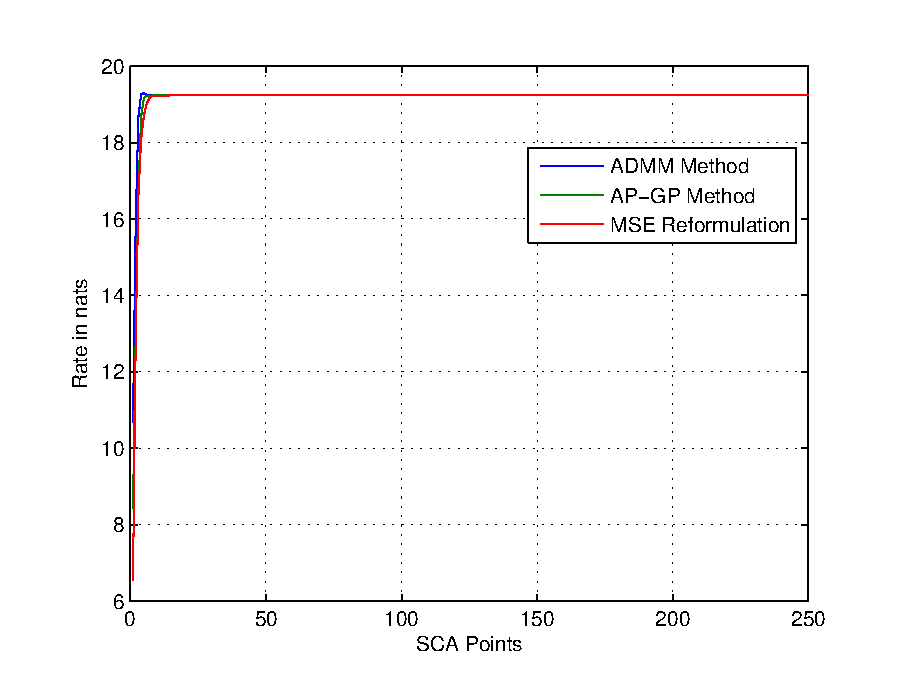
\includegraphics[width=0.75\textwidth]{plot8142}
		\caption{Convergence of sum rate with $N_\mathrm{T} = 8, B = 2, K = 4$, Mobile users}
		\label{fig_1}
	\end{subfigure}
	\begin{subfigure}[b]{0.75\textwidth}
		\centering
		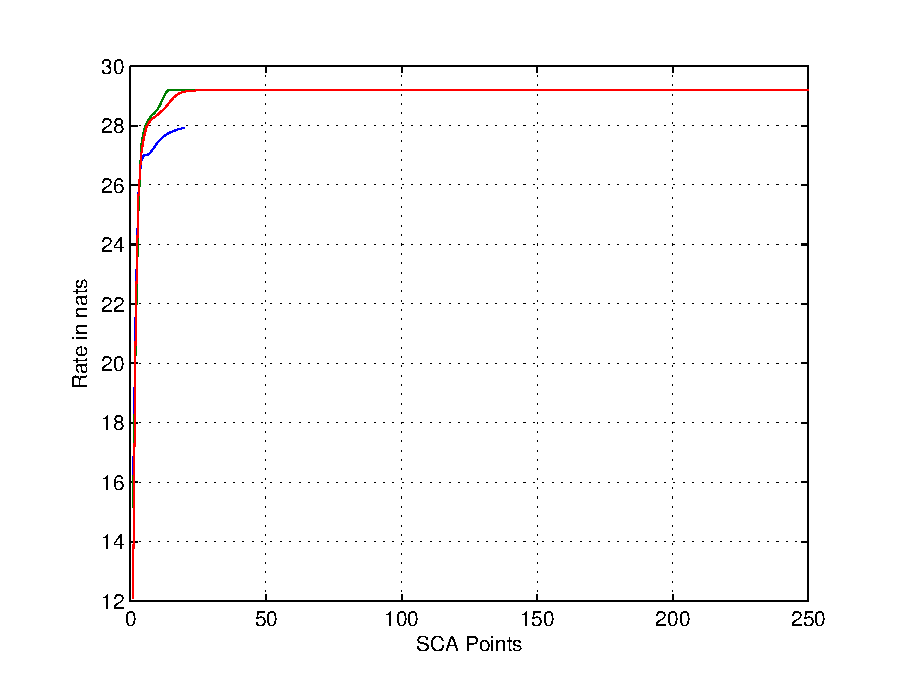
\includegraphics[width=0.75\textwidth]{plot8182}
		\caption{Convergence of sum rate with $N_\mathrm{T} = 8, B = 2, K = 8$, Mobile users}
		\label{fig-2}
	\end{subfigure}
	\caption{Sum rate convergence for mobile users}
	\label{figII}
\end{figure}


\begin{figure}
	\centering
	\begin{subfigure}[b]{0.75\textwidth}
		\centering
		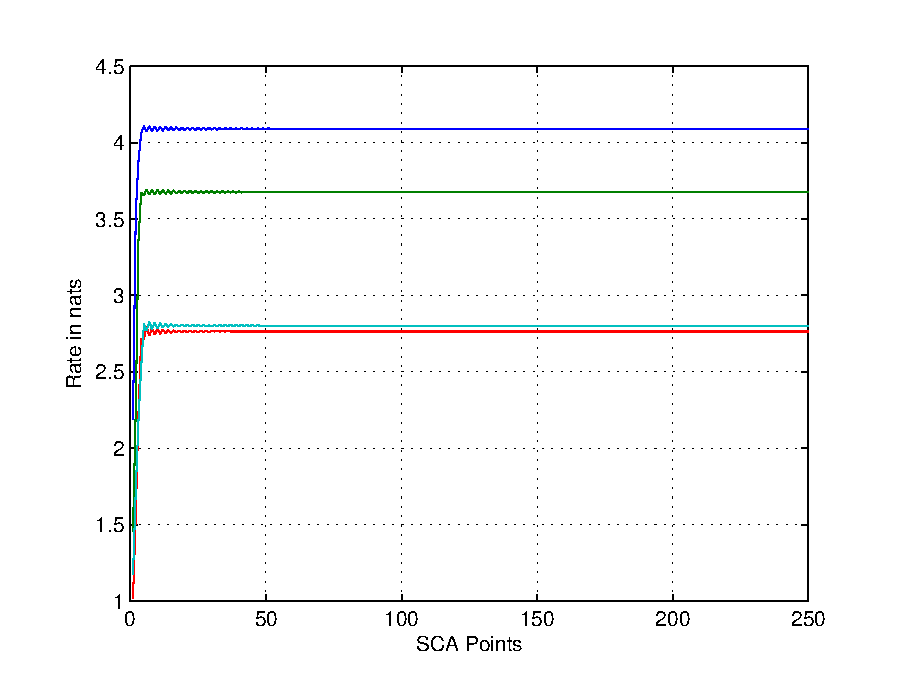
\includegraphics[width=0.75\textwidth]{kktrc8142}
		\caption{Convergence of sum rate with $N_\mathrm{T} = 8, B = 2, K = 4$, Mobile users}
		\label{fig_1}
	\end{subfigure}
	\begin{subfigure}[b]{0.75\textwidth}
		\centering
		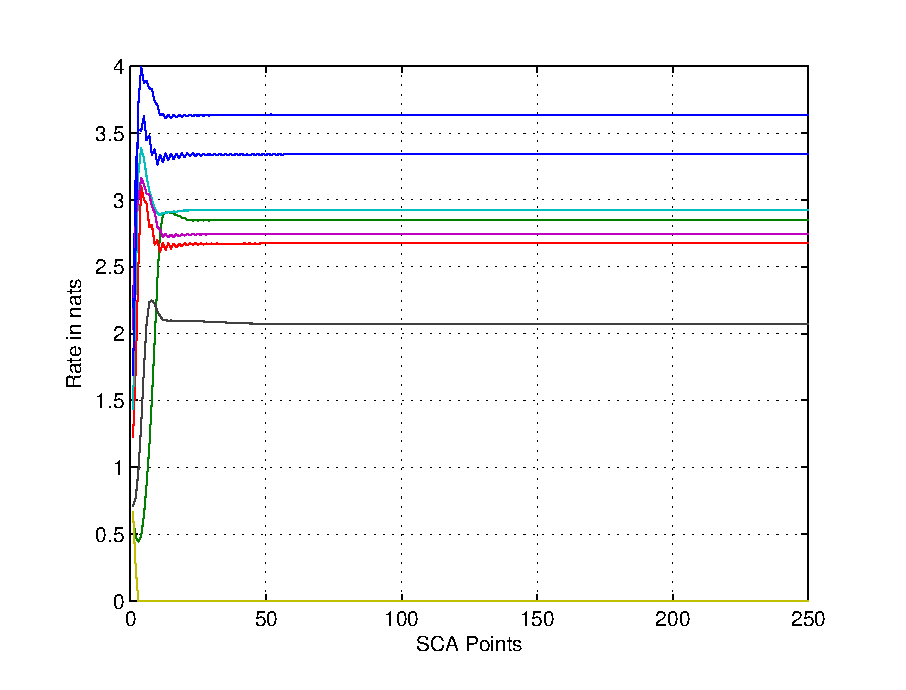
\includegraphics[width=0.75\textwidth]{kkte0rc8182}
		\caption{Convergence of sum rate with $N_\mathrm{T} = 8, B = 2, K = 8$, Mobile users}
		\label{fig-2}
	\end{subfigure}
	\caption{Sum rate convergence for mobile users}
	\label{figII}
\end{figure}

\begin{figure}
	\centering
	\begin{subfigure}[b]{0.75\textwidth}
		\centering
		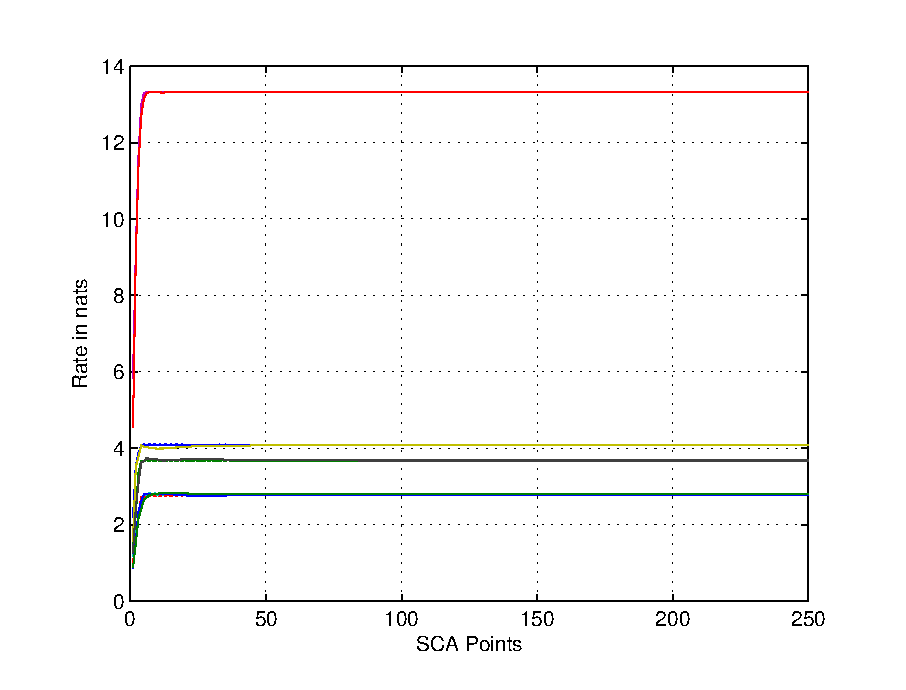
\includegraphics[width=0.75\textwidth]{kktmserc8142}
		\caption{Convergence of sum rate with $N_\mathrm{T} = 8, B = 2, K = 4$, Mobile users}
		\label{fig_1}
	\end{subfigure}
	\begin{subfigure}[b]{0.75\textwidth}
		\centering
		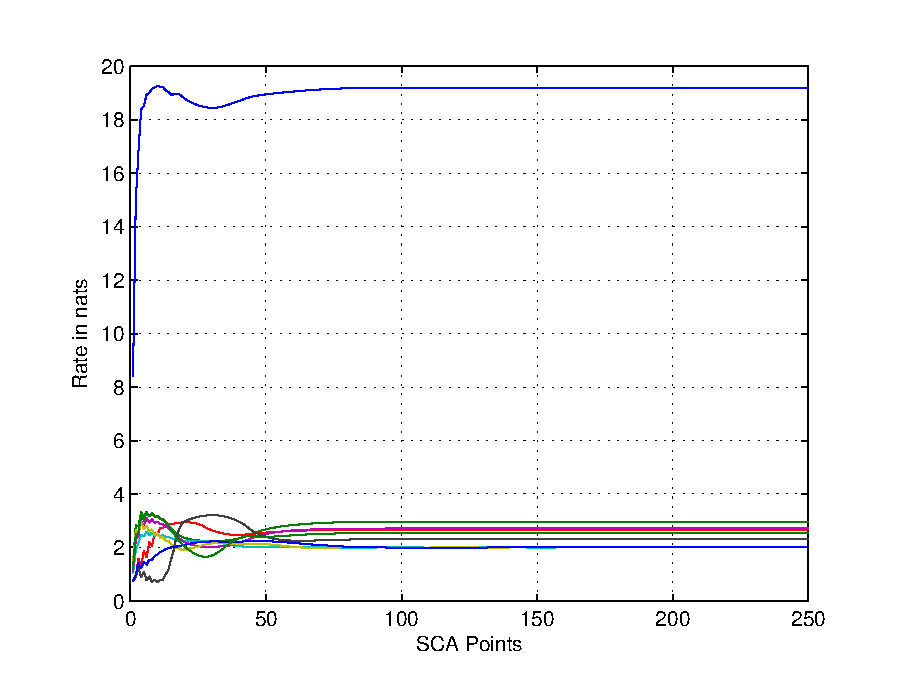
\includegraphics[width=0.75\textwidth]{kktmserc8182}
		\caption{Convergence of sum rate with $N_\mathrm{T} = 8, B = 2, K = $, Mobile users}
		\label{fig-2}
	\end{subfigure}
	\caption{Sum rate convergence for mobile users}
	\label{figIII}
\end{figure}

%\begin{figure}
%\centering
%\begin{subfigure}[b]{0.75\textwidth}
%\centering
%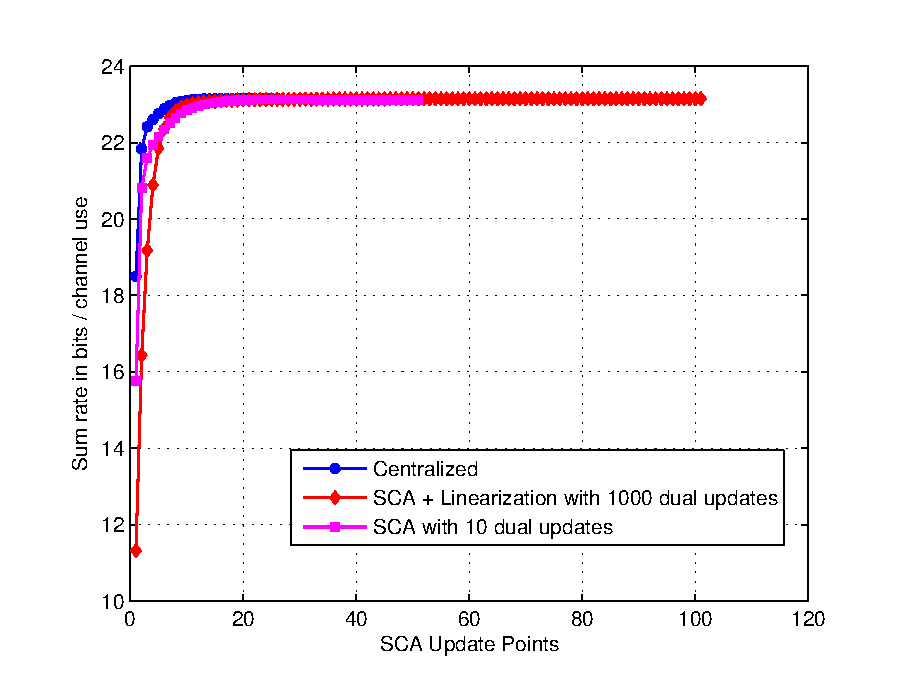
\includegraphics[width=0.75\textwidth]{2_6_8_1}
%\caption{Convergence of sum rate with $N_\mathrm{T} = 8, B = 2, K = 6$, Mobile users}
%\label{fig_1}
%\end{subfigure}
%\begin{subfigure}[b]{0.75\textwidth}
%\centering
%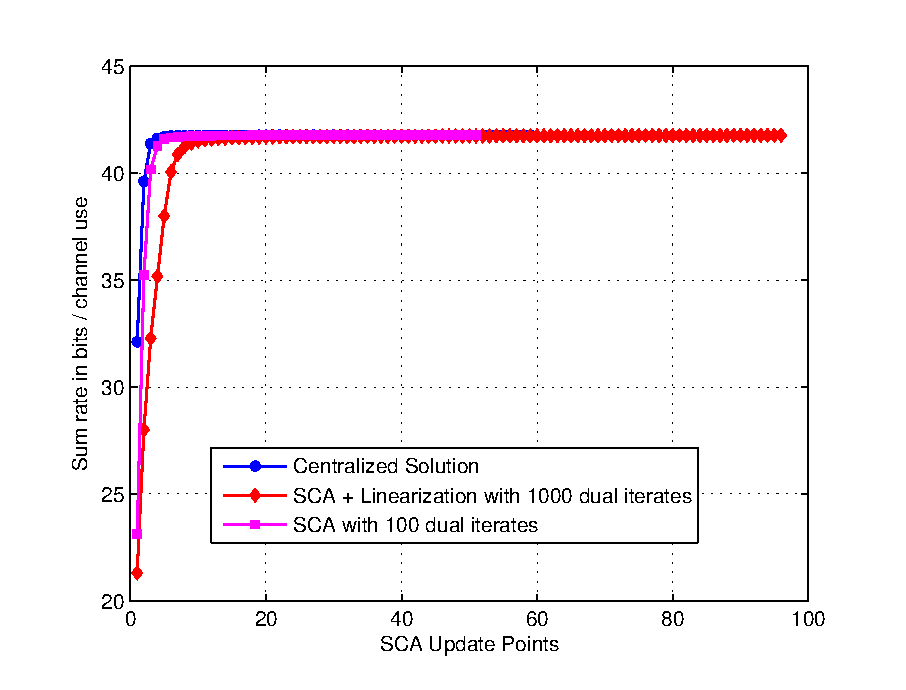
\includegraphics[width=0.75\textwidth]{3_9_12_1}
%\caption{Convergence of sum rate with $N_\mathrm{T} = 12, B = 3, K = 9$, Mobile users}
%\label{fig-2}
%\end{subfigure}
%\caption{Sum rate convergence for mobile users}
%\label{figIV}
%\end{figure}

\newpage

 

\newpage

\chapter{\huge Summary and Conclusions}

In this Thesis Report, we have discussed the 
\newpage

 

\appendix

\chapter{Convergence Proof for Centralized Algorithm}


\chapter{Convergence Proof for Distributed Algorithm}

The convergence of the distributed algorithms as proposed in Algorithm 1, Algorithm 2 and Algorithm 3 follows the same discussion as in Convergence proof for centralized algorithm, if the sub problem in (4.1) converges to the centralized solution. Slater's condition is a sufficient condition for strong duality to hold for a convex optimization problem, Slater's condition states that the feasible region must have an interior point which is satisfied by (4.1) where, by having a non empty set interior and a compact set as required for the convergence 'reference'. Let us consider each distributed algorithms into our convergence analysis. 

In Primal decomposition, the master subproblem uses subgradient to update the coupling variable (interference vectors) in consensus with the objective function, the convergence of the sub problem is gauranteed as the iteration index tends to infinite for a diminishing step size parameter 'reference'.

In \ac{ADMM} method, we prove the convergence by considering the problem discussed in 'reference'  \me{'boydhttps://web.stanford.edu/~boyd/papers/pdf/admm_slides.pdf'}  by writing the problem as
\begin{subeqnarray}
\underset{x, z}{\text{maximize}} \quad && f(x) + g(z) \\
{\text{subject to}} && Ax = z \\
&& x \, \in \mathbb{C}_1, z \, \in \mathbb{C}_2 
\end{subeqnarray}

%write abt ADMM

Let us consider the decomposition via \ac{KKT} conditions for AP-GP method without rate constraint, presented in section 2.A, updates all the optimization variables at once








\chapter{KKT condition for AP-GP method and MSE Reformulation with and without Rate Constraint}

In order to solve for an iterative precoder design algorithm, the \ac{KKT} expressions for the problem in \eqref{APGP_eqn} and \eqref{apgprc_eqn} are obtained by differentiating the Lagrangian by assuming their constraint.

\section{AP-GP without Rate Constraint}

By differentiating the Lagrangian by assuming the equality constraint for \eqref{APGP_eqn}. At stationary points, the following conditions are satisfied.

\begin{subeqnarray}
&&\nabla_{\gamma_k} \,: \, -\dfrac{-\log_2 e}{1 + \gamma_k} + \dfrac{a_k}{2 \phi_k} \, = \, 0 \\
&&\nabla_{\beta_k}\, : \, -\dfrac{a_k \phi_k}{2} - b_k\, = \, 0 \\
&&\nabla_{\mathbf{w}_k} \,: 2 \mathbf{w}_k \left(\sum_{i \neq K} b_i \mathbf{h}_{{b_k},i}^H \mathbf{h}_{{b_k},i}  + c_k \mathbf{I}_{N_T} \; \right )\, = \, a_k \mathbf{h}_{{b_k},k}^H.
\end{subeqnarray}	

Along with the primal constraints given in \eqref{APGP_eqn}, the complementary slackness must also be satisfied at stationary point. On solving the above equations in (7.1) with the complementary slackness conditions, we get an iterative algorithm for finding the transmit beamformer as shown in \eqref{APGP_kkt}.

\section{AP-GP with Rate Constraint}

By differentiating the Lagrangian by assuming the equality constraint for \eqref{APGP_eqn} and \eqref{apgprc2_eqn}. At stationary points, the following conditions are satisfied.

\begin{subeqnarray}
&&\nabla_{\gamma_k} \,: \,  \dfrac{a_k}{2 \phi_k} - \dfrac{1}{1 - \gamma_k} - d_k \, = \, 0 \\
&&\nabla_{\beta_k}\, : \, -\dfrac{a_k \phi_k}{2} - b_k\, = \, 0 \\
&&\nabla_{\mathbf{w}_k} \,: 2 \mathbf{w}_k \left(\sum_{i \neq K} b_i \mathbf{h}_{{b_k},i}^H \mathbf{h}_{{b_k},i}  + c_k \mathbf{I}_{N_T} \; \right )\, = \, a_k \mathbf{h}_{{b_k},k}^H.
\end{subeqnarray}	

Along with the primal constraints given in \eqref{APGP_eqn} and \eqref{apgprc2_eqn}, the complementary slackness must also be satisfied at stationary point. On solving the above equations in (7.2) with the complementary slackness conditions, we get an iterative algorithm for finding the transmit beamformer as shown in \eqref{apgprckkt_eqn}.

\newpage

\section{MSE with Rate Constraint}

By differentiating the Lagrangian by assuming the equality constraint for \eqref{kktmse2_eqn}. At stationary points, the following conditions are satisfied.

\begin{subeqnarray}
&&\nabla_{\epsilon_k} \,: \, \dfrac{1}{\bar{\epsilon_k}} - a_k  \, = \, 0 \\
&&\nabla_{\mathbf{w}_k} \,:  \mathbf{w}_k \left(a_k \sum_{i \neq K}  \mathbf{h}_{{b_k},i}^H \mathbf{u}_i^H \mathbf{u}_i \mathbf{h}_{{b_k},i}  + b_k \mathbf{I}_{N_T} \; \right )\, = \, a_k \mathbf{u}_k^H \mathbf{h}_{{b_k},k}.
\end{subeqnarray}	

Along with the primal constraints given in \eqref{kktmse2_eqn}, the complementary slackness must also be satisfied at stationary point. On solving the above equations in (7.3) with the complementary slackness conditions, we get an iterative algorithm for finding the transmit beamformer as shown in \eqref{kktmse4_eqn}.

\section{MSE with Rate Constraint}

In order to solve for an iterative precoder design algorithm, the \ac{KKT} expressions for the problem in \eqref{kktmse2_eqn} and \eqref{kktmserc1a_eqn} are obtained by differentiating the Lagrangian by assuming their constraint.

\begin{subeqnarray}
&&\nabla_{\epsilon_k} \,: \, \dfrac{1}{\bar{\epsilon_k}} - \dfrac{c_k}{\log \bar{\epsilon_k}} - a_k  \, = \, 0 \\
&&\nabla_{\mathbf{w}_k} \,:  \mathbf{w}_k \left(a_k \sum_{i \neq K}  \mathbf{h}_{{b_k},i}^H \mathbf{u}_i^H \mathbf{u}_i \mathbf{h}_{{b_k},i}  + b_k \mathbf{I}_{N_T} \; \right )\, = \, a_k \mathbf{u}_k^H \mathbf{h}_{{b_k},k}.
\end{subeqnarray}	

Along with the primal constraints given in \eqref{kktmse2_eqn} and \eqref{kktmserc1a_eqn}, the complementary slackness must also be satisfied at stationary point. On solving the above equations in (7.4) with the complementary slackness conditions, we get an iterative algorithm for finding the transmit beamformer as shown in \eqref{kktmserckkt_eqn}.

\chapter{\huge Reference}
%\bibliographystyle{unsrt}
%\bibliography{reference}

\newpage

 

\newpage



\end{document} 